%%%%%%%%%%%%%%%%%%%%%%%%%%%%%%%%%%%%%%%%%
% Masters/Doctoral Thesis 
% LaTeX Template
% Version 2.4 (22/11/16)
%
% This template has been downloaded from:
% http://www.LaTeXTemplates.com
%
% Version 2.x major modifications by:
% Vel (vel@latextemplates.com)
%
% This template is based on a template by:
% Steve Gunn (http://users.ecs.soton.ac.uk/srg/softwaretools/document/templates/)
% Sunil Patel (http://www.sunilpatel.co.uk/thesis-template/)
%
% Template license:
% CC BY-NC-SA 3.0 (http://creativecommons.org/licenses/by-nc-sa/3.0/)
%
%%%%%%%%%%%%%%%%%%%%%%%%%%%%%%%%%%%%%%%%%

%----------------------------------------------------------------------------------------
%	PACKAGES AND OTHER DOCUMENT CONFIGURATIONS
%----------------------------------------------------------------------------------------


\documentclass[
11pt, % The default document font size, options: 10pt, 11pt, 12pt
oneside, % Two side (alternating margins) for binding by default, uncomment to switch to one side
ngerman, 
singlespacing, % Single line spacing, alternatives: onehalfspacing or doublespacing
%draft, % Uncomment to enable draft mode (no pictures, no links, overfull hboxes indicated)
%nolistspacing, % If the document is onehalfspacing or doublespacing, uncomment this to set spacing in lists to single
%liststotoc, % Uncomment to add the list of figures/tables/etc to the table of contents
%toctotoc, % Uncomment to add the main table of contents to the table of contents
parskip, % Uncomment to add space between paragraphs
%nohyperref, % Uncomment to not load the hyperref package
headsepline, % Uncomment to get a line under the header
chapterinoneline, % Uncomment to place the chapter title next to the number on one line
%consistentlayout, % Uncomment to change the layout of the declaration, abstract and acknowledgements pages to match the default layout
]{MastersDoctoralThesis} % The class file specifying the document structure

\usepackage[utf8]{inputenc} % Required for inputting international characters
\usepackage[T1]{fontenc} % Output font encoding for international characters

\usepackage{palatino} % Use the Palatino font by default

\usepackage[backend=bibtex,style=numeric,natbib=true]{biblatex} % Use the bibtex backend with the authoryear citation style (which resembles APA)

\addbibresource{bibliography.bib} % The filename of the bibliography

\usepackage[autostyle=true]{csquotes} % Required to generate language-dependent quotes in the bibliography

\usepackage{microtype}
\usepackage{pdfpages}
\usepackage{graphicx}
\usepackage[font=it]{caption}

\usepackage{listings}
\lstdefinelanguage{VHDL}{
   morekeywords={
     library,use,all,entity,is,port,in,out,end,architecture,of,
     begin,and
   },
   morecomment=[l]--
}

\lstdefinestyle{vhdl}{
   language     = VHDL,
   basicstyle   = \ttfamily,
   keywordstyle = \color{keyword}\bfseries,
   commentstyle = \color{comment}
}

% command \code{Text}
%\newcommand{\code}[1]{\texttt{#1}}

%----------------------------------------------------------------------------------------
%	MARGIN SETTINGS
%----------------------------------------------------------------------------------------

\geometry{
	paper=a4paper, % Change to letterpaper for US letter
	inner=2.5cm, % Inner margin
	outer=3.8cm, % Outer margin
	bindingoffset=.5cm, % Binding offset
	top=1.5cm, % Top margin
	bottom=1.5cm, % Bottom margin
	%showframe, % Uncomment to show how the type block is set on the page
}

%----------------------------------------------------------------------------------------
%	THESIS INFORMATION
%----------------------------------------------------------------------------------------

\thesistitle{Implementierung der RISC-V Spezifikation auf einem FPGA in VHDL} % Your thesis title, this is used in the title and abstract, print it elsewhere with \ttitle
\supervisor{Prof. Dr. \textsc{Reith}} % Your supervisor's name, this is used in the title page, print it elsewhere with \supname
\examiner{} % Your examiner's name, this is not currently used anywhere in the template, print it elsewhere with \examname
\degree{} % Your degree name, this is used in the title page and abstract, print it elsewhere with \degreename
\author{Andreas \textsc{Rollbühler},\\ Jens \textsc{Nazarenus},\\ Nils \textsc{Geiselhart}} % Your name, this is used in the title page and abstract, print it elsewhere with \authorname
\addresses{} % Your address, this is not currently used anywhere in the template, print it elsewhere with \addressname

\subject{Informatik} % Your subject area, this is not currently used anywhere in the template, print it elsewhere with \subjectname
\keywords{} % Keywords for your thesis, this is not currently used anywhere in the template, print it elsewhere with \keywordnames
\university{\href{https://www.hs-rm.de/de/}{Hochschule RheinMain}} % Your university's name and URL, this is used in the title page and abstract, print it elsewhere with \univname
\department{\href{https://www.hs-rm.de/de/fachbereiche/design-informatik-medien/aktuelles/}{Fachbereich Design Informatik Medien}} % Your department's name and URL, this is used in the title page and abstract, print it elsewhere with \deptname
\group{\href{}{}} % Your research group's name and URL, this is used in the title page, print it elsewhere with \groupname
\faculty{\href{}{}} % Your faculty's name and URL, this is used in the title page and abstract, print it elsewhere with \facname

\AtBeginDocument{
\hypersetup{pdftitle=\ttitle} % Set the PDF's title to your title
\hypersetup{pdfauthor=\authorname} % Set the PDF's author to your name
\hypersetup{pdfkeywords=\keywordnames} % Set the PDF's keywords to your keywords
}

\begin{document}

\frontmatter % Use roman page numbering style (i, ii, iii, iv...) for the pre-content pages

\pagestyle{plain} % Default to the plain heading style until the thesis style is called for the body content

%----------------------------------------------------------------------------------------
%	TITLE PAGE
%----------------------------------------------------------------------------------------

\begin{titlepage}
\begin{center}

\vspace*{.06\textheight}
{\scshape\LARGE \univname\par}\vspace{1.5cm} % University name
\textsc{\Large Projektdokumentation}\\[0.5cm] % Thesis type

\HRule \\[0.4cm] % Horizontal line
{\huge \bfseries \ttitle\par}\vspace{0.4cm} % Thesis title
\HRule \\[1.5cm] % Horizontal line
 
\begin{minipage}[t]{0.4\textwidth}

\begin{flushleft} \large
\emph{Autoren:}\\
\authorname % Author name - remove the \href bracket to remove the link
\end{flushleft}
\end{minipage}
\begin{minipage}[t]{0.4\textwidth}
\begin{flushright} \large
\emph{Projektbetreuer:} \\
\href{https://www.cs.hs-rm.de/~reith/}{\supname} % Supervisor name - remove the \href bracket to remove the link  
\end{flushright}
\end{minipage}\\[3cm]
 
\vfill

\large \textit{Dokumentation der Praktischen Tätigkeit\\ im Rahmen des Wahlprojekts Hardware/Software-Schnittstellen\\ im Wintersemester 2016/1017}
\\[1cm] % University requirement text
%\textit{im}\\[0.4cm]
%\groupname\\\deptname\\[2cm] % Research group name and department name
 
\vfill

{\large \today}\\[2cm] % Date


\includegraphics[scale=0.8]{HSRM_logo} % University/department logo - uncomment to place it
 
\vfill
\end{center}
\end{titlepage}

%----------------------------------------------------------------------------------------
%	ABSTRACT PAGE
%----------------------------------------------------------------------------------------

\begin{abstract}
\addchaptertocentry{\abstractname} % Add the abstract to the table of contents

Dieses Dokument wurde im Rahmen des Wahlprojekts \textit{Software- Hardwareschnittstellen} bei Prof. Dr. \emph{Reith} an der Hochschule RheinMain verfasst. 

Es dokumentiert die Konzeptionalisierung und die Implementierung einer CPU auf einem \textit{FPGA} Board. Die verwendete Befehlssatzarchitektur basiert auf dem offenen \textit{\href{https://riscv.org/}{RISC-V}} Design. Die Architektur wurde unter Verwendung der Hardwarebeschreibungssprache \textit{VHDL} implementiert. Anschließend wurde sie testweise für das \textit{\href{https://reference.digilentinc.com/reference/programmable-logic/nexys-4/start}{Xilinx Nexys 4\textsuperscript{\textregistered}}} Board mit Artix-7\textsuperscript{\textregistered} \emph{FPGA} synthetisiert.

Ferner dokumentiert diese Arbeit das Projekt- und Teammanagement. Sie beschreibt die Verwendung von Versionskontrollsystemen, den Workflow und die Testumgebung im Zusammenhang mit der VHDL-Entwicklungsumgebung \textit{Xilinx} \textit{\href{https://www.xilinx.com/products/design-tools/vivado.html}{Vivado\textsuperscript{\textregistered} Design Suite}}.

Das umgesetzte Projekt ist unter der GPL3-Lizenz veröffentlicht und das Repository \ref{???} frei verfügbar.
 
\end{abstract}

%----------------------------------------------------------------------------------------
%	LIST OF CONTENTS
%----------------------------------------------------------------------------------------

\let\cleardoublepage\clearpage 
\tableofcontents % Prints the main table of contents

%\listoffigures % Prints the list of figures

%\listoftables % Prints the list of tables

%----------------------------------------------------------------------------------------
%	THESIS CONTENT - CHAPTERS
%----------------------------------------------------------------------------------------

\mainmatter % Begin numeric (1,2,3...) page numbering

\pagestyle{thesis} % Return the page headers back to the "thesis" style

% Include the chapters of the thesis as separate files from the Chapters folder
% Uncomment the lines as you write the chapters

\chapter{Einleitung} % Main chapter title
\label{Einleitung} % For referencing the chapter elsewhere, use \ref{Chapter1} 

%----------------------------------------------------------------------------------------

% Define some commands to keep the formatting separated from the content 
\newcommand{\keyword}[1]{\textbf{#1}}
\newcommand{\tabhead}[1]{\textbf{#1}}
\newcommand{\code}[1]{\texttt{#1}}
\newcommand{\file}[1]{\texttt{\bfseries#1}}
\newcommand{\option}[1]{\itshape#1}

Diese Arbeit wurde im Rahmen des Wahlprojekts \textit{Software- Hardwareschnittstellen} bei Prof. Dr. \emph{Reith} an der Hochschule RheinMain verfasst. Die vorgegebene Projektaufgabe beinhaltet die Implementierung einer CPU auf einem \emph{FPGA} mittels der Hardwarebeschreibungssprache \emph{VHDL}. Die CPU soll die offene \emph{RISV-V} Architektur umsetzen. Diese Dokumentation beschreibt das Konzept, die Planung und die Umsetzung dieser Aufgabenstellung.

Zunächst werden hierfür einige allgemeine Grundbegriffe, die zum Verständnis des Projekts erforderlich sind, kurz erläutert: Die FPGA-Technologie, die Hardwarebeschreibungssprache VHDL, die offene Befehlssatzarchitektur RISC-V und welche Teilmenge des (modularen) RISC-V Befehlssatzes umgesetzt wurde. Dabei soll jedoch lediglich ein kurzer Überblick über die Materie verschafft werden. Für das tiefere Verständnis und Anleitungen sei auf die entsprechende Fachliteratur für VHDL\citep{Ashenden:609207}, FPGA-Programmierung\cite{Chu} mit Vivado\cite{churiwala} und auf die RISC-V Spezifikation\citep{RISC} verwiesen.

Der Schwerpunkt liegt stattdessen auf der Beschreibung der Umsetzung der gesetzten Aufgabenstellung. Dafür wurde in Kapitel \ref{Umsetzung} die konkrete Implementierung der einzelnen Komponenten der RISC-V CPU in VHDL dokumentiert. Anschließend stellt Kapitel \ref{organisation} die Herausforderungen des Team- und Projektmanangements dar und wie mit ihnen umgegangen wurde. Es wird die Arbeitsteilung, die Versionskontrolle mit \emph{git} und die Qualitätssicherung durch Softwaretests beschrieben.

Kapitel \ref{Probleme} dokumentiert die Herausforderungen, auf die das Team im Laufe der Entwicklung gestoßen ist und inwiefern dadurch Teile der Umsetzung limitiert oder eingeschränkt werden mussten. Es werden außerdem mögliche Lösungsansätze diskutiert. Ferner wird ein kurzer Ausblick auf künftige Entwicklungen des Projekts gegeben.

Schließlich werden in Kapitel \ref{Ergebnis} die Ergebnisse der Arbeit zusammengefasst dargestellt und die Details und Kennwerte der umgesetzten CPU aufbereitet. 

Das Ergebnis dieser Arbeit ist unter \ref{???} frei verfügbar.
 %Einleitung
\chapter{FPGA} % Main chapter title
\label{FPGA} % For referencing the chapter elsewhere, use \ref{Chapter1} 

Ein FPGA (Field Programmable Gate Array) ist ein Schaltkreis, in den eine beliebige logische Schaltung programmiert werden kann. Der Vorteil besteht dabei insbesondere darin, dass FPGA's beliebig oft neu programmiert werden können. 

%----------------------------------------------------------------------------------------
\section{Technik}

%---------------------------------------------------------------------------------------- %FPGA
\chapter{VHDL} % Main chapter title
\label{VHDL} % For referencing the chapter elsewhere, use \ref{Chapter1} 

%----------------------------------------------------------------------------------------
\section{Einleitung}
VHDL (\textit{Very High Speed Integrated Circuit Hardware Description Language}) ist eine Hardwarebeschreibungssprache, die 1980 entwickelt wurde. Mit ihr kann das Verhalten einer logischen Schaltung formal beschrieben werden. \cite[S. 22f.]{kesel2013entwurf}

Anstatt eine Schaltung aus ihren einzelnen elektronischen Bauteilen zu entwerfen, arbeitet VHDL aber auf einer höheren Abstraktionsschicht. Es wird lediglich beschrieben, wie sich eine Schaltung oder ein logischer Teil einer Schaltung in Abhängigkeit bestimmter Eingangsgrößen verhält.
%----------------------------------------------------------------------------------------

%----------------------------------------------------------------------------------------
\section{Entwicklung mit VHDL}
\paragraph{Entities.} In VHDL werden \textit{Entities} definiert, die eine Klasse von Schaltelementen repräsentieren. Entities bestehen üblicherweise aus mehreren Ein-und Ausgangs\textit{ports}. Innerhalb einer Entity wird ihre \emph{Architecture} beschrieben. Diese kann entweder ihr Verhalten als innere Funktion oder ihre Struktur beschreiben.

\paragraph{Architecture.} Im \emph{Verhaltensmodell} einer Entity wird definiert, wie sich die Ausgangssignale in Abhängigkeit der Eingangssignale verhalten.

Um komplexe Schaltungen hierarchisch zu gliedern, kann die Architecture auch als \emph{Strukturmodell} beschrieben werden. Hier wird auf übergeordneter Ebene die Verschaltung mehrerer Subkomponenten definiert. Dafür werden Instanzen von zuvor beschriebenen Entities (sog. \textit{Components}) erstellt und deren Ports miteinander verbunden. \cite[S. 25ff.]{kesel2013entwurf}

\paragraph{Parallelität.} Bei der Entwicklung ist insbesondere zu beachten, dass das Verhalten einer Entity, anders als von Programmiersprachen gewohnt, im Allgemeinen nicht sequentiell abgearbeitet wird. Vielmehr findet die Signalverarbeitung parallel statt.

\paragraph{Prozesse.} Innerhalb des Verhaltens können deshalb Prozesse deklariert werden, deren Instruktionen sequentiell abgearbeitet werden. Zu diesem Zweck können innerhalb eines Prozesses auch \textit{Variablen} verwendet werden. \cite[S. 29f.]{kesel2013entwurf}
%----------------------------------------------------------------------------------------
 
%----------------------------------------------------------------------------------------
\section{Umsetzung von VHDL}
Auf die konkrete Umsetzung der beschriebenen Schaltung hat der Anwender dabei nur bedingten Einfluss, da die Implementierung der Schaltung in Hardware selbst üblicherweise von automatisierten Werkzeugen durchgeführt wird. Dabei lassen sich mehrere Schritte unterscheiden. In diesem Projekt wurde die Entwicklungsumgebung Vivado Design Suite von Xilinx verwendet, um den VHDL-Code umzusetzen.

\paragraph{Simulation.} In einem ersten Schritt kann das Verhalten des VHDL Codes \emph{simuliert} werden, was vor allem in der Testphase von Bedeutung ist. Dabei wird der Code noch nicht auf der Hardware ausgeführt, sondern das Verhalten der Schaltung mittels sogenannter Testbenches simuliert, die die Schaltung mit virtuellen Eingangssignalen (z. B. Taktrate) versorgen. \cite[S. 81]{SynthesisFPGA} \ref{testbench}

\begin{figure} [ht]
  \centering
  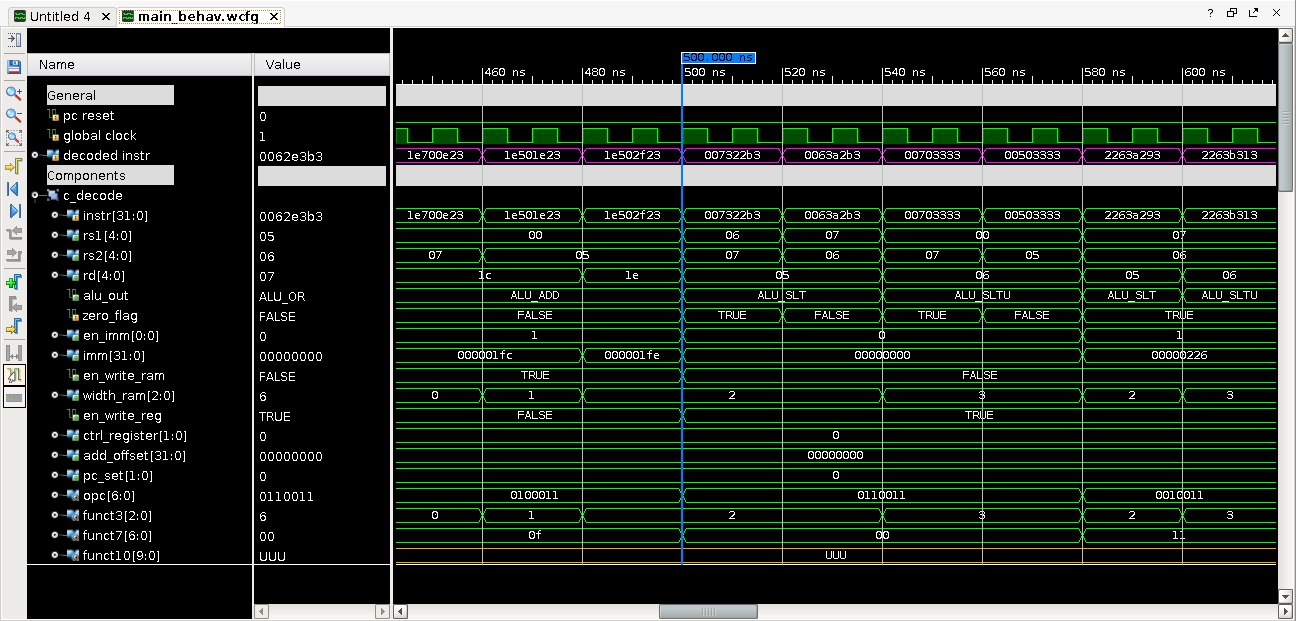
\includegraphics[width=\textwidth]{Figures/simulation}
  \caption{Beispiel für die Simulation einer komplexen Schaltung mit Vivado Design Suite: Zu sehen ist die graphische Darstellung von Signalen in Abhängigkeit der Zeitkomponente}
  \label{fig:simulation}
\end{figure}

\paragraph{Synthese.} Das simulierte Verhalten kann anschließend \emph{synthetisiert} werden. Dabei ist zu beachten, dass nicht die vollständige Menge von zulässigem (und simulationsfähigem) VHDL-Code letztlich in eine physische Schaltung synthetisierbar ist (so z. B. \emph{wait}-Statements). Das ist abhängig von der verwendeten Zieltechnologie (FPGA, ASIC) und dem verwendeten Synthesewerkzeug. Das Ergebnis der Synthese ist eine (hardwareunabhängige) Netzliste, die einer textuellen Beschreibung des umgesetzten Schaltplans entspricht.

\paragraph{Implementierung.} Diese Netzliste ist Grundlage der Hardwareimplementierung. Dabei wird innerhalb des \emph{place and route} Vorgangs unter Berücksichtigung der verfügbaren Hardware und bestimmter zeitlicher Beschränkungen berechnet, wo die einzelnen Schaltelemente auf der Hardware implementiert werden und wie sie verbunden werden. Dabei wird ein Bitstream generiert, der anschließend auf die Hardware geladen werden kann. \cite[S. 21]{SynthesisFPGA}
%----------------------------------------------------------------------------------------
 %VHDL
\chapter{RISC-V} % Main chapter title
\label{RISC-V} % For referencing the chapter elsewhere, use \ref{Chapter1} 

\section{Einleitung}
\emph{RISC-V} ist eine offene Befehlssatzarchitektur, die 2010 von
Entwicklern an der University of California, Berkeley vorgestellt wurde.
Sie liegt derzeit in Version 2.1 vor (\textit{Stand: März 2017}). RISC-V
basiert auf der RISC (reduced instruction set computing) Designphilosophie.

\paragraph{RISC.} Der Grundgedanke von RISC-Architekturen ist, dass ein Maschinenbefehl möglichst wenige Taktzyklen in der Ausführung benötigt. Damit grenzt sich RISC zu CISC (complex instruction set computing)-Systemen ab, die komplexe Instruktionen beinhalten und zum Teil viele Taktzyklen zur Ausführung benötigen können. RISC-Programme bestehen daher üblicherweise aus mehr Maschinenbefehlen, die aber tendenziell schneller abgearbeitet werden.

Auch wenn der Begriff \textit{reduced instruction} sich
eigentlich nicht auf die Menge der verfügbaren Maschineninstruktionen
bezieht, bestehen RISC-Designs in der Praxis dennoch meist aus weniger
Maschinenbefehlen. Außerdem erfordern RISC-Architekturen in der Regel eine weniger komplizierte Verschaltung. \cite{DBLP:conf/sipew/IsenJJ09} Der Vorteil von RISC-Designs ist somit, insbesondere im Hinblick auf dieses Projekt, dass sie einfacher zu implementieren sind.

%----------------------------------------------------------------------------------------
\section{Architektur}
\label{subsec:Register}

\paragraph{Speicherarchitektur.} RISC-V ist als
\textit{load-store}-Architektur entworfen. Arithmetische und logische
Instruktionen greifen daher nicht auf den Speicher zu, stattdessen
werden alle Operanden und Operationsergebnisse in der Registerbank
abgelegt zwischengespeichert.
Speicherzugriffe werden ausschließlich mit speziellen \textit{Load}- bzw. \textit{Store}-Befehlen realisiert.

\paragraph{Register.} Die RISC-V-Spezifikation definiert $31$
Integer-Register $x1 - x31$. Zusätzlich existiert das
\textit{zero}-Register $x0$, das konstant mit dem Wert $0$ belegt ist. RISC-V-Register sind beliebig verwendbare General-Purpose-Register, die sowohl für Daten als auch Adressen vorgesehen sind. Besondere Verwendungen einzelner Register sind lediglich durch Programmierkonventionen beschrieben. Sonstige Register (v. a. Floating-Point-Register) sind für spezielle Befehlssatzerweiterungen vorgesehen, werden aber an dieser Stelle vernachlässigt.

\paragraph{Instruktionslänge.} RISC-V-Maschinenbefehle sind, wie bei
RISC üblich, in einer fixen Länge kodiert. Sie entspricht der Wortbreite
der Prozessorarchitektur. Für RISC-V-Architekturen sind die Wortbreiten
$32, 64$ oder $128$-Bit vorgesehen.

\paragraph{Byte-Order.} Die RISC-V-Architektur verwendet Little-Endian-Kodierung.
%----------------------------------------------------------------------------------------

%----------------------------------------------------------------------------------------
\section{RISC-V-Varianten}
\label{sec:erweiterung}

\paragraph{Erweiterbarkeit.} Die RISC-V-Architektur ist darauf ausgelegt, flexibel erweiterbar zu sein. Die Spezifikation definiert daher mehrere Teilmengen des Befehlssatzes. \cite[p. 4]{RISC}

\paragraph{Mindeststandard.} Um die RISC-V-Anforderungen zu erfüllen,
muss eine Implementierung zumindest den Basisbefehlssatz umsetzen
(Bezeichnung nach \mbox{RISC-V}-Konvention: \textit{I}). Dieser enthält
neben Befehlen zur Integer-Arithmetik auch Integer Load- und Store-Befehle, sowie die notwendigen Befehle zur Manipulation des Kontrollflusses.

\paragraph{Erweiterungen.} Die allgemeine -- als \textit{General
Purpose} bezeichnete -- Architektur enthält neben diesem Mindeststandard auch Befehle für Gleitkommaarithmetik (F) mit Double (D) oder Quad-Präzision (Q), für die Handhabung verschiedener Privilegierungen (P), für die Verwaltung von Nebenläufigkeit (A) und seit der neusten Version 2.1 auch für Bitmanipulation (B), Vectoroperationen (V) und einigen mehr. \cite[p. 4f.]{RISC}

\paragraph{Umgesetzte Instruktionsmenge.} In diesem Projekt wurde sich
allerdings darauf beschränkt, eine einfache integerverarbeitende
Mikroarchitektur umzusetzen. Als Wortbreite wurde 32-Bit gewählt. Die Bezeichnung des verwendeten Subsets lautet daher nach RISC-V-Konvention \textit{RV32I}. \cite[p. 67ff.]{RISC}
%----------------------------------------------------------------------------------------

%----------------------------------------------------------------------------------------
\section{RV32I}
Das verwendete Subset besteht aus insgesamt $47$ verschiedenen
Maschineninstruktionen. Neben Instruktionen zur Integer-Arithmetik, sind dabei Branch-Instruktionen und Speicherzugriffe enthalten.

\subsection{Instruktionsformate}
RV32I kennt vier verschiedene Typen, in denen Maschineninstruktionen
enkodiert sein können: \textit{R-type}, \textit{I-Type}, \textit{S-type}
und \textit{U-type} - Befehle (siehe Abbildung \ref{fig:instr_types}).
Dabei sind Opcode, sowie Ausgangsregister ($rs1$, $rs2$) und
Zielregister ($rd$) der Operationen immer an der gleichen Stelle des
Maschinenbefehls kodiert. Sofern ein konstanter Wert (\emph{Immediate})
in der Instruktion enthalten ist, ist dieser jeweils in den
höchstwertigst verfügbaren Bits der Instruktion enkodiert. Die Einteilung in 
Instruktionstypen erleichtert die Dekodierung der Instruktionen und führt zu einer simpleren Verschaltung.

\begin{itemize}  
\item Als R-Type sind Register-Instruktionen enkodiert, bei denen beide Operanden in Registern liegen. 
\item Die I-Type-Kodierung ist für Instruktionen vorgesehen, bei denen ein konstanter Wert (\textit{Immediate}) mit einem Wert im Register verrechnet wird.
\item U-Type Befehle umfassen bedingte und unbedingte Sprungbefehle.
\item Der S-Type wird für schreibende Zugriffe auf den Speicher (store) verwendet. 
\end{itemize}

\begin{figure} [h]
  \centering
  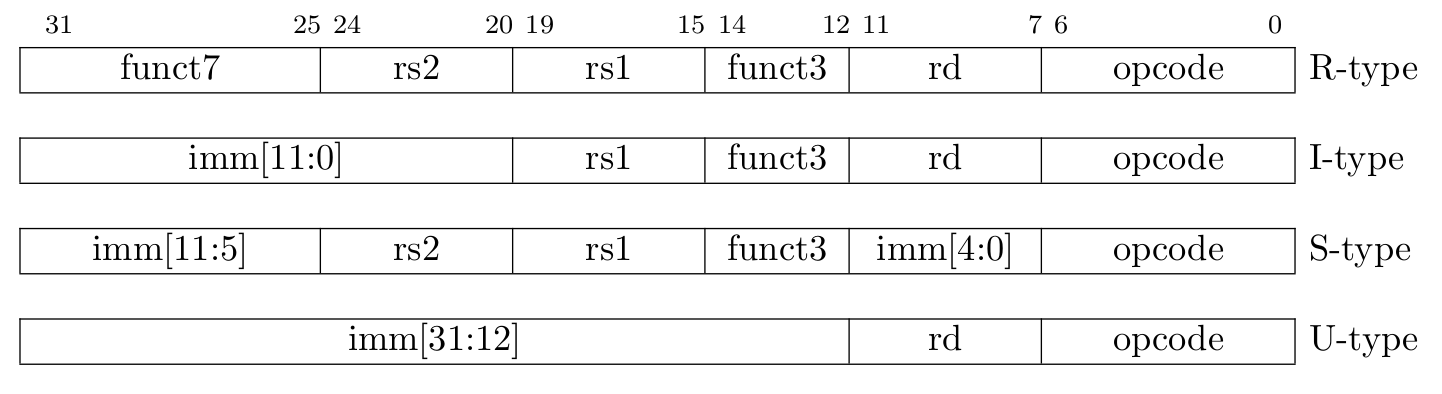
\includegraphics[width=\textwidth]{Figures/instruction_formats}
  \caption{Instruktionsformate. Quelle: \citep[S. 11]{RISC}}
  \label{fig:instr_types}
\end{figure}

\subsection{Immediate-Varianten.} Außerdem existieren mehrere Varianten,
um Immediates aus den Instruktionen zu extrahieren (siehe Abbildung
\ref{fig:immediates}). Diese unterschiedlichen Kodierungen sind ebenfalls so gewählt, um die Überschneidungen der einzelnen Formate zu maximieren und dadurch die Implementierung zu vereinfachen. \cite[S. 11f.]{RISC} 

\begin{figure} [ht]
  \centering
  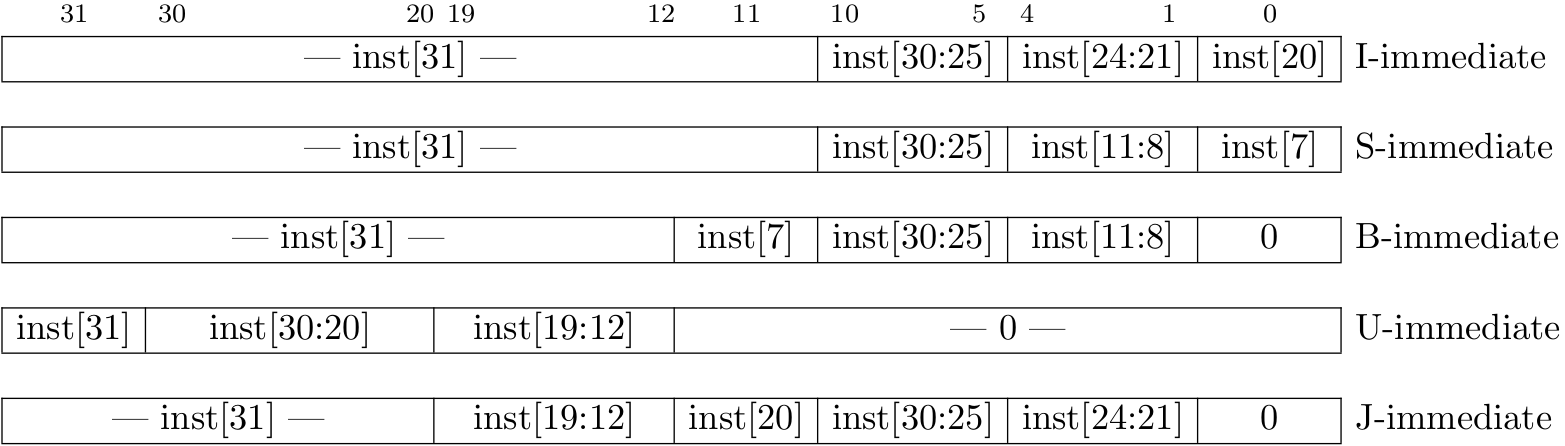
\includegraphics[width=\textwidth]{Figures/immediates}
  \caption{Immediateenkodierungen. Quelle: \citep[S. 12]{RISC}}
  \label{fig:immediates}
\end{figure}

\subsection{Einzelne Instruktionen}
Die in dieser Arbeit umgesetzten Instruktionen des RV32I-Standards können im einzelnen der Tabelle in Anhang \ref{Maschinenbefehle} entnommen werden. Im Folgenden soll lediglich ein Überblick über die Instruktionen dargestellt werden. Ferner wird die Kodierung eines Maschinenbefehls exemplarisch im Detail besprochen.

\paragraph{Integer-Arithmetik.}
Bei integerverarbeitenden Instruktionen kann unterschieden werden zwischen solchen, die eine Operation auf zwei Registerwerten ausführen (als R-Type kodiert) und solchen, die eine Operation auf einem Registerwert und einem Immediate (I-Type) ausführen. Das Operationsergebnis wird jeweils im Zielregister ($rd$) gespeichert.

In den \emph{funct3}- bzw. \emph{funct7}-Bits ist die Operation kodiert,
die auf den Operanden angewendet werden soll. RISC-V definiert
arithmetische Operationen wie die Addition (\emph{ADDI} bzw. \emph{ADD})
und Bitshift-Operationen (\textit{SLL, SRL, SRA}). Außerdem sind
vergleichende Operationen, z. B. Kleiner-Als (\textit{SLT}) vorgesehen,
die eine $1$ im Zielregister ablegt, wenn die Bedingung erfüllt ist,
dass der \emph{rs1}-Registerwert kleiner als der \emph{rs2}-Registerwert
ist. Schließlich sind logische Bitoperationen (\textit{AND, OR, XOR}) definiert.

Es ist außerdem der spezielle \textit{LUI}-Befehl vorgesehen, der
benötigt wird, um 32-Bit-Konstanten in ein Register zu laden. Aufgrund
der festen Instruktionslänge von 32-Bit kann keine ganze
32-Bit-Immediate in einer Instruktion kodiert werden. \textit{LUI} füllt 
deshalb nur die höchstwertigsten 20 Bit eines Wertes und belegt den Rest mit $0$. In einem 
zweiten Schritt kann dann durch eine Veroderung mit dem \textit{ORI}-Befehl der restliche Teil nachgeladen werden.

\paragraph{Beispiel.} In Abbildung \ref{fig:addi} ist exemplarisch der \textit{ADDI}-Befehl zu sehen. Dieser soll einen im Maschinenbefehl kodierten Immediate-Wert mit einem Wert in einem bestimmten Register addieren und das Ergebnis anschließend in einem Zielregister speichern.
 
Dafür ist in der Maschineninstruktion der Opcode $0010011$ (Bit $6 -
0$) kodiert, der die Information enthält, dass eine Immediate-Operation durchgeführt werden soll. Die Bits 14-12 kodieren, die die auszuführende Rechenoperation beschreibt (hier: $000$ für die Addition). Ferner ist das Zielregister $rd$, das Ausgangsregister $rs1$ und der Immediate-Wert (Bit $31 - 20$) im Maschinenbefehl selbst kodiert.

\begin{figure} [ht]
  \centering
  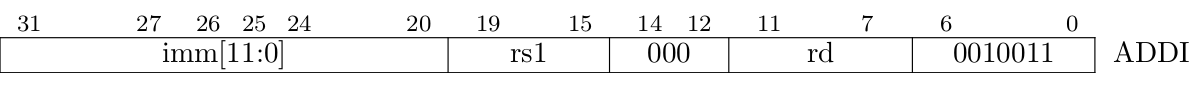
\includegraphics[width=\textwidth]{Figures/ADDI}
  \caption{ADDI-Instruktion.}
  \label{fig:addi}
\end{figure}

\paragraph{Kontrollfluss.}
Um die Reihenfolge, mit der die Maschinenbefehle ausgeführt werden zu
manipulieren, existieren bedingte Sprungbefehle (\textit{BEQ, BNE, BLT,
BGE}). Diese führen einen relativen Sprung an einen Offset von der aktuellen
Adresse des Programmzählers aus, wenn eine bestimmte Bedingung
erfüllt ist, z. B. wenn die Registerinhalte \emph{rs1} und \emph{rs2} gleich sind.

Außerdem existieren unbedingte Sprungbefehle (\textit{JAL, JALR}), die
vor allem zum Aufruf von Subroutinen erforderlich sind. \emph{JAL}
springt ebenfalls den in der Immediate kodierten Offset der aktuellen
Adresse an und speichert
die folgende Maschinenbefehladresse im Zielregister \emph{rd}, um später
wieder zurückkehren zu können. \emph{JALR} springt dagegen eine absolute
Adresse an, die aus dem Immediate-Wert und dem Register \emph{rs1} errechnet wird.

\paragraph{Speicherzugriffe.}
Da RISC-V als Load-Store-Architektur entworfen ist, sind Zugriffe auf den Speicher nur in speziellen Load-/Store-Befehlen vorgesehen. Die \textit{load}-Instruktion lädt einen Wert aus dem Speicher in ein Register, die \textit{store}-Instruktion schreibt einen Registerinhalt an eine bestimmte Speicheradresse. RISC-V erlaubt dabei Zugriffe auf einzelne Byte, Halfwords (2 Byte) und Words (4 Byte).
%----------------------------------------------------------------------------------------

 %RISC
\iffalse
Herausforderungen:
\TODO: ELF, 


Sonstiges:
\TODO: links zu Quellcode
\TODO: Warnings entfernen
\fi

\chapter{Umsetzung} % Main chapter title
\label{Umsetzung} % For referencing the chapter elsewhere, use \ref{Chapter1} 

%----------------------------------------------------------------------------------------
\section{Komponenten der CPU}

Unter Anhang~\ref{schaltplan} findet man einen skizzenhaften Aufbau der CPU, der die einzelnen Komponenten und deren Verbindungen untereinander darstellt.
Diese Skizze wurde während der Implementierungsphase sukzessive erweitert und stellte ein wichtiges Hilfsmittel dar, das erheblich zur Übersicht und zum Verständnis über das Zusammenwirkens der Bauteile beigetragen hat.
In vorliegendem Kapitel sollen die Funktionsweise und der Aufbau der einzelnen Komponenten und einige implementierungsspezifische Details erläutert werden.

\subsection{Decode}

In dieser Komponente wird der aktuelle Maschinenbefehl, nachdem er aus dem Speicher geladen wurde, dekodiert und die daraus gewonnenen Informationen werden über Steuersignale an die jeweiligen Einheiten der CPU übertragen:
\begin{itemize}
    \item Die \textit{Registerbank} bekommt mitgeteilt, welche Registerinhalte sie an ihre Ausgänge anlegen soll und in welches Register ein potentielles Ergebnis geschrieben werden muss.
        Außerdem wird über einen \textit{Multiplexer} gesteuert, ob dieses Ergebnis vom \textit{Program Counter}, dem \textit{Hauptspeicher} oder der \textit{ALU} zu erwarten ist.
    \item An die \textit{ALU} wird der Operationstyp übermittelt, den diese auf ihre beiden Operanden anwendet.
        Zusätzlich wird auch hier ein Multiplexer angesteuert, der der ALU entweder einen Registerinhalt oder eine Konstante als zweiten Operanden zuweist.
    \item Der \textit{Hauptspeicher} erhält Informationen über die Bitbreite und die Art eines Speicherzugriffs (lesend/schreibend).
    \item Der Wert des \textit{Program Counters} muss bei Sprungbefehlen angepasst werden.
\end{itemize}
Es werden also alle Informationen, die zur Ausführung eines Maschinenbefehls nötig sind, von der Dekodiereinheit extrahiert und an die zugehörige Stelle übertragen. 

Bei der Umsetzung dieser Aufgabe erweist sich der Aufbau der Maschinenbefehle (siehe Anhang~\ref{Maschinenbefehle}) als sehr hilfreich:
Vergleichbare Informationen belegen innerhalb der 32-Bit- Instruktionen die gleichen Positionen.
Enthält ein Maschinenbefehl z.B. ein Zielregister in das ein Ergebnis geschrieben werden soll, so befindet sich die Adresse dieses Zielrgisters an der gleichen Position, an der es sich auch bei anderen Befehlen befindet.
Das erleichtert zum einen die Implementierung, da einem Ausgangsport über mehrer Befehle hinweg die gleichen Bits eines Eingangsports zugeordnet werden können, und verringert zum anderen die Komplexität der daraus resultierenden Schaltungen. 
Ein Blick in den Quellcode (siehe~\ref{}) zeigt, dass eine verschachtelte \textit{Case}-Abfrage den Ausgangsports die passenden Signale zuweist, die ohne den vorteilhaften Aufbau der Maschinenbefehle wesentlich komplexer geraten wäre.

\subsection{Program Counter}

Beim sog. \textit{Program Counter} (kurz: \textit{PC}) handelt es sich um ein flankengesteuertes 32-Bit-Register mit asynchronem Reset, das die Adresse enthält, unter der der nächste abzuarbeitende Maschinenbefehl im Hauptspeicher zu finden ist. 
Wie der Name schon vermuten lässt, ist der PC als Zählregister implementiert:
Alle zwei Takte wird der aktuelle Registerwert um vier erhöht, um damit den nächsten 32-Bit-Maschinenbefehl zu adressieren.
Ein Flag (\textit{enable}), das nur alle zwei Takte gesetzt ist, verhindert, dass dieser Vorgang jeden Takt zur Ausführung kommt.

Soll ein Sprungbefehl ausgeführt werden, muss der Wert des PCs auf eine neue Adresse gesetzt oder ein Offset auf den aktuellen Zählerstand addiert werden.
Beide Funktionialitäten wurden direkt im PC implementiert, um einen Umweg über die \textit{ALU} zu vermeiden.
Hierfür stehen die Eingangsports \textit{set}, \textit{set\_value} und \textit{set\_jalr} zur Verfügung.

Am Ausgangsport \textit{value\_out\_next} liegt die Adresse des nächsten Maschinenbefehls (\textit{PC + 4}) an, die als Rücksprungadresse optional in der Registerbank abgespeichert werden kann, um zu einem späteren Zeitpunkt zum ürsprünglichen Ausführungsstrang zurückkehren zu können.

Die Implementierung des Program Counters unterliegt den Prinzipien des \textit{synchronen Designs}:~\cite[S. 72 ff.]{Chu}
Der nächste Registerwert wird unabhängig vom Taktsignal berechnet (\textit{cnt\_next}) und dem Ausgangsport erst bei steigender Taktflanke zugewiesen. 

\subsection{Registerbank}

Bevor die CPU eine Rechenoperationen durchführen kann, müssen die passenden Operanden aus dem Hauptspeicher geladen und in der \textit{Registerbank} zwischengespeichert werden.
Diese besteht aus 32 Registern der Länge 32 Bit, wobei es sich bei der vorliegenden Implementierung eigentlich um ein Array aus nur 31 Registern handelt, da das \textit{Register 0} konstant den Wert $0$ enthält und nicht überschrieben werden kann~(\ref{subsec:Register}).

Ein asynchroner Leseprozess versorgt die beiden Datenausgänge mit den Inhalten der beiden Register, die durch die Eingänge \textit{rs1} und \textit{rs2} ausgewählt werden.
Beide Ausgänge leiten die Werte an die ALU weiter, während eine zusätzliche Verbindung zum RAM die Ausführung einer \textit{Store}-Instruktion erleichtert.
Ein Schreibprozess in das Register mit dem Index \textit{rd} ist nur bei steigender Taktflanke und gleichzeitig gesetztem Eingangsport \textit{en\_write} möglich, womit ein unkontrolliertes Speichern verhindert wird.
Dieser Vorgang benötigt zwei Takte, da bei steigender Taktflanke des ersten Taktes noch nicht gewährleistet werden kann, dass alle Signale in definiertem Zustand anliegen.
Der Dateneingang kann mittels eines vorgeschalteten Multiplexers Werte aus den RAM, der ALU oder dem PC empfangen.



\subsection{Arithmetisch Logische Einheit}

Die eigentlichen Rechenoperationen werden in der arithmetisch-logischen Einheit (kurz: \textit{ALU} für \textit{arithmetic logic unit}) durchgeführt.
Wie der Name bereits andeutet, führt diese Einheit arithmetische und logische Funktionen auf zwei 32-Bit-Zahlen aus.
Neben den beiden Dateneingängen enthält die ALU einen weiteren Eingang (\textit{op\_in}), über den sie von der Decode-Einheit den auszuführenden Funktionstypen erhält.
Das Ergebnis der Berechnung wird, abhängig vom Maschinenbefehl, entweder an die Registerbank, den Hauptspeicher oder den Program Counter weitergeleitet.
Ein weiterer Ausgangsport (\textit{zero\_flag}) versorgt die Dekodiereinheit bei bedingten Sprungbefehlen mit der Information, ob ein Sprung genommen werden muss. 

Bei der Implementierung wurde eine einfache \textit{Case}-Anweisung verwendet, die den Funktionstypen abfragt, woraufhin die entsprechende Funktion zur Anwendung kommt.

\subsection{Random Access Memory}
\label{subsec:RAM}

Im \textit{RAM} (kurz für: \textit{Random Access Memory}, auch \textit{Hauptspeicher} genannt), werden die Maschinenbefehle und sonstige, zur Programmausführung benötigte Daten, abgespeichert.
Für die Erstellung dieser Komponente gibt es eine Reihe von vorgegebenen Templates an die man sich halten sollte, wenn man sicherstellen möchte, dass die Synthese das gewünschte Ergebnis liefert.~\cite[S. 243 ff.]{Chu}

Grundsätzlich unterscheidet man zwei Arten von RAM, die auf dem vorliegenden FPGA implementiert werden können:
Während der sog. \textit{Distributed RAM} auf die Look-Up-Tables und Logigblöcke des FPGAs zugreift, handelt es sich beim sog. \textit{Block RAM} um ein internes Speichermodul des FPGAs~\ref{}
Benötigt man viel Speicherplatz, ist es ratsam eher den Block RAM zu verwenden, da dieser keine Logikzellen belegt, wohingegen Distributed RAM flexibler konfiguriert werden kann.
Bei resourcen- und zeitkritischeren Projekten bedarf die Entscheidung, welche Art von RAM man letztendlich verwendet, sicherlich einer eingehenden Analyse, bei der vorliegenden Implementierung wurde dies als nicht notwendig erachtet.


In diesem Fall wurde der Hauptspeicher als \textit{Dual-Port RAM} mit \textit{asynchronem Lesezugriff} konfiguriert, was von den Synthesetools automatisch als Distributed RAM erkannt und umgesetzt wird.
Der Begriff Dual-Port bezieht sich auf den Umstand, dass die Komponente je zwei Ein- und Ausgangsports besitzt.
Da zusätzlich zwei separate Adressleitungen zur Verfügung stehen, kann simultan auf Maschinenbefehle und Daten zugegriffen werden.
Somit ist es möglich den aktuell zu bearbeitenden Maschinenbefehl an die Dekodiereinheit weiterzuleiten, ohne diesen in ein Register zwischenzuspeichern und gleichzeitg Daten, die gelesen werden müssen, an den Datenausgang anzulegen.
Die ansychronen Lesezugriffe haben den Vorteil, dass die Daten nach einer kurzen Verzögerung zur Verfügung stehen, anstatt einen weiteren Takt darauf warten zu müssen.
Der Schreibzugriff ist, ähnlich wie bei der Registerbank, taktflankengesteuert und von einem zusätzlichen Flag abhängig.
%TODO: Größe RAM

\paragraph{RAM-Control.} Der RISC-V-Instruktionssatz sieht eine Byte-Adressierung für den Hauptspeicher vor, d.h. mit einer Speicheradresse ist es möglich genau ein Byte zu adressieren.
Zusätzlich erfordern bestimmte Instruktionen, wie z.B. \textit{load halfword} oder \textit{load word} einen Zugriff auf 16 oder 32 Bit.
Möchte man diese Unterscheidung der Bitbreite eines Zugriffs direkt im RAM implementieren, läuft man Gefahr, dass das Ergebnis nicht mehr dem vorgegebenen Template entspricht und der RAM bei der Synthese nicht mehr als solcher erkannt wird.
Aus diesem Grund wurde eine zusätzliche \textit{RAM-Control}-Einheit erstellt, die die Zugriffslogik abstrahiert und sicherstellt, dass auf den Hauptspeicher nur mit der Breite von 32 Bit zugegriffen wird.

\paragraph{Adressierung.} Wird nun ein bestimmtes Byte im Speicher adressiert, muss die Kontrolleinheit die Adresse umwandeln, um die Position des zugehörigen Wortes im RAM zu erhalten. 
Dieses Wort wird anschließend gelesen um daraus über die beiden niederwertigsten Bits der ursprünglichen Adresse das passende Byte zu extrahieren.

Ein Beispiel soll diesen Vorgang verdeutlichen:\\
Angenommen der Hauptspeicher enthält das Wort $00184421_{16}$ an der Adresse $2_{16}$,
und es erfolgt ein Zugriff auf ein Byte über die Adresse $A_{16}$.
\begin{figure} [htpb]
    \centering
        \begin{tabular}{|c|c|c|c|c|}
            \multicolumn{1}{c}{3} & \multicolumn{1}{c}{2} &  \multicolumn{1}{c}{1}& \multicolumn{1}{c}{0}\\
            \hline
            $00_{16}$ & $18_{16}$ & $44_{16}$ & $21_{16}$\\
            \hline
        \end{tabular}
        \caption{Speicherinhalt an der Adresse $2_{16}$}
\end{figure}
\\                                                        
Da sich die Adresse $A_{16}$ auf ein Byte bezieht, muss sie von der Kontrolleinheit durch vier geteilt werden um an das Wort im Speicher, das das gewünschte Byte enthält, zu gelangen.
Unter der resultierenden Adresse $2_{16}$ wird folglich das oben dargestellte Wort gelesen.
Anschließend wird über die niederwertigsten Bits der ursprünglichen Adresse, in diesem Fall also $10_2$, das passende Byte mit dem Inhalt $18_{16}$ aus diesem Wort extrahiert.\\
Handelt es sich um einen Lesezugriff wird dieses Byte zu einem Wort umgeformt und an den Datenausgang angelegt:\\
\begin{figure} [htpb]
    \centering
        \begin{tabular}{|c|c|c|c|c|}
            \multicolumn{1}{c}{3} & \multicolumn{1}{c}{2} &  \multicolumn{1}{c}{1}& \multicolumn{1}{c}{0}\\
            \hline
            $00_{16}$ & $00_{16}$ & $00_{16}$ & $18_{16}$\\
            \hline
        \end{tabular}
        \caption{Der Wert am Datenausgang nach dem Lesezugriff}
\end{figure}\\
In diesem Fall wird das Wort mit Nullen aufgefüllt. 
Bei einem \textit{sign extended Load}-Befehl kann dies auch mit Einsen geschehen, abhängig vom höchstwertigsten Bit des zu ladenden Byte.

Wird schreibend, z.B. mit dem Wert FF$_{16}$,  auf diese Adresse zugegriffen, muss das Byte $18_{16}$ im ursprünglichen Wort ersetzt und das modifizierte Wort wieder an die Adresse 0x2 in den Speicher zurückgeschrieben werden:
\begin{figure} [htpb]
    \centering
        \begin{tabular}{|c|c|c|c|c|}
            \multicolumn{1}{c}{3} & \multicolumn{1}{c}{2} &  \multicolumn{1}{c}{1}& \multicolumn{1}{c}{0}\\
            \hline
            $00_{16}$ & FF$_{16}$ & $44_{16}$ & $21_{16}$\\
            \hline
        \end{tabular}
        \caption{Speicherinhalt an der Adresse $2_{16}$ nach dem Schreibzugriff}
\end{figure}\\
Dieser Vorgang kommt ebenso bei Speicherzugriffen der Breite 16 Bit zur Anwendung.
Wird dagegen auf ein 32-Bit-Wort zugegriffen, muss lediglich die Adresse übersetzt werden.


%----------------------------------------------------------------------------------------

 %Umsetzung
\chapter{Organisation} 
\label{organisation} 

\section{Teammanagement}
Um das gemeinsame Ziel, nämlich die Implementierung einer RISC-V CPU,
umzusetzen musste vor Beginn der eigentlichen Arbeit gewisse
Vorkehrungen getroffen werden, um die Arbeit im Team zu ermöglichen.
Hierzu gehört insbesondere die Einigung auf eine bestimmte
Projektstruktur und eine Versionsverwaltung in welcher die Quelldateien
der Implementierung abgelegt werden können. Einige dieser
organisatorischen Angelegenheiten werden in den folgenden Kapiteln 
genauer erläutert. 

\subsection{Projektstruktur}
Wie bereits in Kapitel \ref{vivado} erwähnt wurde ist als
Entwicklungsumgebung Vivado zum Einsatz gekommen. Vivado gibt für
VHDL-Projekte bereits eine bestimmte Projektstruktur vor, diese ist
jedoch für die Arbeit im Team ungeeignet, da sie Dateien mit festen 
Pfadangaben  und vielen temporären, automatisch erzeugten Dateien
beinhaltet. Dadurch können Vivado-Projekte nicht ohne Weiteres in einer
gemeinsamen Versionsverwaltung geteilt werden. Um trotz allem eine
Projektstruktur zu erstellen, die auch für das Versionskontrollsystem
\emph{git} geeignet ist, sind verschiedene Anpassungen nötig gewesen.

\paragraph{Build-Script.}  
Vivado selbst ist in der Programmiersprache Tcl geschrieben und kann
ebenfalls mit dieser Programmiersprache erweitert werden. Es ist möglich
ein Tcl-Script zu erstellen, was ein temporäres Vivado-Projekt erstellt
in dem gearbeitet werden kann. Der Vorteil ist, dass die Quelldateien in
einem anderen Ordner aufbewahrt werden und unnötige Dateien des
temporären Vivado-Projektes nicht unter Versionskontrolle gestellt werden.

\paragraph{Aufbau.} Es ergibt sich folgende Projektstruktur. Alle Ordner
bis auf \code{work/} werden in einem Versionskontrollsystem abgelegt:
\begin{lstlisting}[inputencoding={utf8},extendedchars=false,escapeinside=``]
riscv/
  documentation/ -- Verzeichnis f`ü`r Dokumentation
  script/        -- Verschiedene Hilfsprogramme 
  src/           -- VHDL Quelldateien 
  test/          -- VHDL Testbench Dateien 
  work/          -- tempor`ä`res Vivado-Projekt (nicht in git) 
  build.sh       -- Programm zur Generierung des Vivado-Projekts
  build.tcl      -- Tcl Script zur Generierung des Vivado-Projekts
  start.sh       -- Start-Programm f`ü`r Vivado 
\end{lstlisting}


\subsection{Versionskontrolle}
Als Versionsverwaltungssystem hat sich die Gruppe für \emph{git}
entschieden. Die Hochschule RheinMain bietet für Softwareprojekte
zusätzlich einen \emph{Gitlab}-Server an, auf dem das Projekt unter
dem Namen
\textbf{vhdl-cpu/riscv}\footnote{\url{https://zenon.cs.hs-rm.de/vhdl-cpu/riscv}
(08.03.2017)} geführt ist.

\subsection{Arbeitsweise}

\paragraph{Workflow.} Das Projekt wurde unter Berücksichtigung des sogenannten
\emph{GitHub-Flows}\footnote{\url{https://guides.github.com/introduction/flow/}
(08.03.2017)}
entwickelt. Das bedeutet, dass verschiedene Regeln, was das 
Versionskontrollsystem betrifft, eingehalten wurden:

\begin{enumerate}
\item Es gibt einen Branch \emph{master}, der zu jeder Zeit kompilierbar
und in Vivado simulierbar ist.
\item Entwicklungen werden in neuen Branches durchgeführt (sogenannte
Feature-Branches).
\item Ist die Entwicklung eines Features für das Projekt abgeschlossen
wird ein \emph{Merge-Request} des entsprechenden Entwicklers gestellt.
\item Die Gruppe entscheidet anschließend gemeinsam, ob das Feature in
den \emph{master}-Branch übernommen werden soll oder, ob noch Änderungen
zur Fertigstellung notwendig sind.
\end{enumerate}

Die Entwicklung nach diesem Prinzip hat mehrere Vorteile. Es ist zum
Beispiel direkt nachvollziehbar wer, welche Teile der Entwicklung
übernommen hat. Auch das gemeinsame Entscheiden über die Integration in
den \emph{master}-Branch kann helfen Fehler frühzeitig zu erkennen.

Zur Synthese der RISC-V-CPU auf dem FPGA wurde zusätzlich noch ein Branch
namens \emph{master\_\,fpga} angelegt. Dieser Branch enthält zusätzlich zu
der CPU noch FPGA-spezifische Änderungen, wie zum Beispiel die
Constraint-Datei für die Portbelegung.

\paragraph{Arbeitsteilung.} In Kapitel \ref{sec:komponenten} wurden die
verschiedenen Komponenten der CPU vorgestellt. Die Entwicklung der
einzelnen Bausteine wurde in der Gruppe aufgeteilt. Anschließend mussten
die verschiedenen Maschinenbefehle, wie in Tabelle
\ref{maschinenbefehle} zu sehen, umgesetzt werden. Diese wurden
nach der Entwicklung der Komponenten aufgeteilt und in Feature-Branches 
entwickelt. Zum Beispiel gibt es einen Branch namens \emph{ar\_\,load}, der die 
Entwicklung der Load/Store-Befehle wie \code{lw, lb, lh} beinhaltet.

\section{Testumgebung} 
\subsection{Testbenches}
Zu jeder erstellten Komponente, die in Kapitel \ref{sec:komponente}
erläutert wurde sind Testbenches erstellt worden. Eine Testbench testet
\emph{eine} Komponente unabhängig und stellt somit einen Modultest der
entsprechenden Komponente dar. Zusätzlich wurde eine Testbench namens
\code{main\_tb} erzeugt, die das Zusammenspiel der einzelnen Komponenten
testet (Integrationstest). In der Testbench \code{main\_tb} kann somit
die Arbeitsweise der CPU simuliert und untersucht werden. 

Generell wurden Testbenches während der Entwicklung verwendet, um zu
überprüfen, ob sich die Signale und Funktionsweise der Komponenten
richtig verhalten.
\subsection{White-Box-Test}
Zusätzlich wurden mehrere White-Box-Tests durchgeführt, mit welchen
ersichtlich ist, ob die CPU die gewünschten Änderungen an den 
Registern nach Abarbeitung einer Instruktion durchführt.

\begin{table}[h]
\centering
\begin{tabular}{|l|l|l|l|}
Instruktion & x5(t0) & x6(t1) & x7(t2) \cr
\hline
lhu t1,506(zero) & 0x81 & 0x8713 & 0x82070785 \cr
add t2, t0, t1 & 0x81 & 0x8713 & 0x8794 \cr 
sub t2,t0,t1 & 0x81 & 0x8713 & 0xffff796e \cr 
xor t2,t0,t1 & 0x81 & 0x8713 & 0x8792 \cr
\dots & \dots & \dots & \dots
\end{tabular}
\caption{Ausschnitt der White-Box-Tests und die Beschreibung der
Register nachdem der entsprechende Test durchgeführt wurde.}
\label{tab:whiteboxtest}
\end{table}
Die Testfälle wurde manuell in der Simulationsansicht von Vivado überprüft.

\subsection{Black-Box-Test}
Nachdem die Implementierung abgeschlossen war und es möglich war den
vorliegenden FPGA mit der RISC-V-CPU zu „programmieren“ wurden
Black-Box-Tests mit dem FPGA durchgeführt. Die niederwertigsten 16 Bits
des Registers \code{a0} (Status-Register) wurden mit den LEDs auf dem FPGA verbunden. Es
wurden verschiedene Programme ausgeführt und die Ausgabe der LED-Anzeige
überprüft.

\subsection{Hilfsprogramm \emph{riscv-instr}}
Um gültige 32 Bit Maschinenbefehle für die CPU testweise zu erstellen
wurde ein Hilfsprogramm namens \emph{riscv-instr} erstellt, welches in
der Lage ist zu einem gültigen Assemblerprogramm die entsprechenden
Instruktionen für die CPU auszugeben. Mit diesem Programm ist es somit
möglich Instruktionen zu erzeugen, die in den RAM der CPU geladen werden
können.

Beispiel-Assembler-Programm:
\begin{lstlisting}
  .globl main
  .type main, @function
main:
  addi x1,x2,12 
  add  x1,x1,x2
\end{lstlisting}

Nach Programmaufruf werden die beiden Instruktionen als Hexadezimal
ausgegeben:
\begin{lstlisting}[language=bash]
riscv-instr testasm.s
0x00c10093 
0x002080b3 
\end{lstlisting}
Die beiden Instruktionen können in den RAM der CPU geladen werden und
können von der RISC-V CPU verarbeitet werden. Das Programm
\emph{riscv-instr} benötigt zur Erzeugung der Maschinenbefehle die 
entsprechende GNU Cross Compiler Toolchain für RISC-V
\footnote{\url{https://github.com/riscv/riscv-gnu-toolchain}
(08.03.2017)}. 

\subsection{RAM-Initialisierung}
Um bei der Erstellung des RAMs möglichst flexibel zu sein kann der
Inhalt aus einer Datei eingelesen werden. \cite[S. 187]{XST}
Hierzu müssen alle Instruktion, die in den RAM der CPU geladen werden
sollen, als 32-Bit-Vektor in einer Datei abgelegt werden:

Beispiel-Datei:
\begin{lstlisting}
00000000000000000000001010010011
00000001001000101110010100010011
00000000000001010000000001100111
...
\end{lstlisting}

Die Funktion \ref{src:blockram_read_file} liest beim Synthese-Vorgang
den Inhalt der entsprechenden Datei und füllt den RAM mit den
Instruktionen. Dies war besonders für den Black-Box-Test notwendig.
 %Herangehensweise
\chapter{Herausforderungen und Ausblick} % Main chapter title
\label{Probleme} % For referencing the chapter elsewhere, use \ref{Chapter1} 

\section{Einleitung}

Bei der Umsetzung dieses Projekts haben sich insbesondere aus Perspektive eines Softwareentwicklers einige neue Herausforderungen gestellt, die sich bei der imperativen Programmierung üblicherweise nicht ergeben (z. B. die grundsätzliche parellele Signalverarbeitung).

Auf einige bestimmte Probleme, mit denen das Team konfrontiert wurde, soll an dieser Stelle gesondert eingegangen werden.

Außerdem sind mehrere Wege denkbar, das entwickelte CPU-Design künftig weiterzuentwickeln. Darunter sind solche, die die Funktionalität erweitern und solche, die das bestehende Design optimieren. Auch auf diese möglichen Entwicklungen soll hier ein kurzer Ausblick gegeben werden.

%----------------------------------------------------------------------------------------
\section{RAM}

In Kapitel~\ref{Umsetzung} wurden Aufbau und Funktionsweise des Hauptspeichers und des RAM-Controllers bereits näher erläutert.
An dieser Stelle sollen nun einige Schwierigkeiten, die während der Implementierung auftraten, und die daraus resultierenden Überlegungen beschrieben werden.

\paragraph{Speicherausrichtung.} 
Ein Speicherzugriff auf $N$ Byte gilt als ausgerichtet, wenn die Startadresse dieser $N$ Byte ein ganzzahliges Vielfaches von $N$ ist~\cite[S. 96/97]{Hennessy}.
Findet z.B. ein Speicherzugriff mit der Breite von 32-Bit auf eine Adresse statt, die nicht ausgerichtet ist, die also kein ganzzahliges Vielfaches von 4 ist, ergibt sich folgendes Problem:
Nicht alle vier Byte des gesuchten Wortes befinden sich unter der gleichen (Wort-)Adresse im Speicher und können daher nicht innerhalb eines einzelnen Zugriffs erreicht werden.

Möchte man diese Art Operation unterstützen, wäre es z. B. denkbar, jeden Zugriff, der mehr als ein Byte umfasst, in eine entsprechende Anzahl von Byte-Zugriffen umzuwandeln, was sich allerdings negativ auf die Performance der CPU auswirken würde.
Außerdem garantiert die RISC-V-Spezifikation nur für ausgerichtete Zugriffe Atomarität, wohingegen bei unausgerichteten Zugriffen zusätzliche Vorkehrungen zu treffen sind~\cite[S. 18]{RISC}.

Der vorliegende RAM-Controller unterstützt unausgerichtete Zugriffe nicht, mit dem Vorteil, dass alle Maschinenbefehle nur zwei Takte zur Ausführung benötigen.
Ein entsprechender Speicherzugriff wird hier also unterbunden, d.h. der Maschinenbefehl wird ignoriert und hat keinerlei Auswirkung.

Umgesetzt wurde dies wie folgt:\\
Bei einem nicht ausgerichteten Schreibzugriff wird der Schreibvorgang nicht unterbrochen, allerdings wird in die jeweilige Speicherstelle der ursprünglich dort enthaltene Wert zurückgeschrieben.
Somit wird der Speicher nicht verändert.\\
Wird dagegen lesend auf eine nicht ausgerichtete Adresse zugegriffen, sendet der RAM-Controller über seinen \textit{dsbl\_wr\_reg}-Port ein Signal an den Dekodierer, der diese Information (\textit{en\_write = false}) an die Registerbank weiterleitet und somit einen Schreibzugriff auf das Register unterbindet, in das der zu lesende Wert aus dem RAM ursprünglich geschrieben werden sollte.

\paragraph{Schreibprozess.} 
Da auf den Hauptspeicher nur ein 32-Bit breiter Zugriff möglich ist, muss der RAM-Controller vor einem Schreibzugriff der Breite 8- oder 16-Bit die adressierte Speicherstelle lesen, um diese verändern und anschließend zurückschreiben zu können~(siehe Kapitel \ref{subsec:RAM}).
Herausforderung bei der Umsetzung dieser Maschineninstruktionen war es, diese in zwei Takten durchführen zu können, um die Anzahl der Takte pro Instruktion nicht erhöhen zu müssen.
Abbildung~\ref{fig:write} zeigt beispielhaft, wie ein Schreibprozess in den RAM durchgeführt wird.
Links sieht man die Namen der enstprechenden Ports und Signale, während rechts deren Werte zum jeweiligen Zeitpunkt (siehe Taktsignal \textit{s\_clk}) dargestellt sind.

\begin{figure}[htpb]
    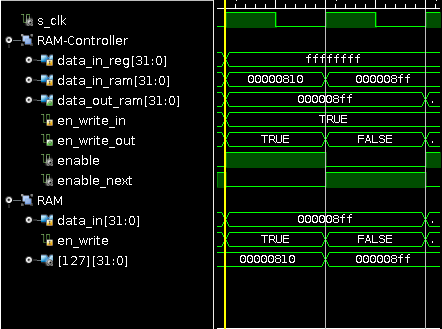
\includegraphics[width=\textwidth]{Figures/write.png}
    \caption{Umsetzung eines Schreibzugriffs in den Speicher}
    \label{fig:write}
\end{figure}

In diesem Beispiel soll ein Byte in den Speicher geschrieben werden:\\
Der RAM-Controller erhält ein Wort von der Registerbank (\textit{data\_in\_reg}), dessen niederwertigstes Byte in den Speicher geschrieben werden soll (in diesem Fall wiederum an die Position des niederwertigsten Bytes).
Gleichzeitig liest er den Wert aus der Speicherstelle, die adressiert wird  (\textit{data\_in\_ram}), um diese mit dem Registerwert zu modifizieren und in den Speicher zurückzuschreiben (\textit{data\_out\_ram}).
Vom Dekoder erhält der RAM-Controller die Information, dass ein Schreibzugriff auf den RAM erforderlich ist (\textit{en\_write\_in}), welche er direkt an den RAM weiterleitet (\textit{en\_write\_out}).
Dieser erhält den Schreibbefehl (\textit{en\_write}) allerdings kurz nach einer steigenden Taktflanke (siehe \textit{s\_clk}), weswegen der eigentliche Schreibvorgang erst im zweiten Takt erfolgt.
Um einen weiteren Schreibzugriff im nächsten Takt zu verhindern, setzt der RAM-Controller das \textit{en\_write\_out}-Signal  mit Hilfe zweier umschaltender Signale (\textit{enable} und \textit{enable\_next}) auf \textit{FALSE}.



\section{Pipelining}
In der vorliegenden Implementierung wurde aus Zeitgründen auf die Umsetzung des sog. Pipelining verzichtet. 
Trotzdem soll hier kurz auf die Grundlagen dieser Technik und deren Voraussetzungen eingegangen werden.
Für eine detaillierte Auseinandersetzung mit diesem Thema wird an dieser Stelle auf weiterführende Literatur verwiesen~\cite[A-2 ff.]{Hennessy}

Pipelining ist ein Verfahren, mit dessen Hilfe die Performance einer CPU verbessert werden kann.
Statt Maschineninstruktionen nacheinander auszuführen, werden diese in Teilaufgaben zerlegt, wodurch es möglich ist, während eines Taktzyklus Befehle parallel abzuarbeiten.
Die Ausführungszeit eines einzelnen Befehls kann dadurch zwar durchaus länger werden, allerdings ist es möglich, insgesamt mehr Instruktionen pro Takt abzuarbeiten.
Klassische Pipeline-Stufen sind z. B.:
\begin{itemize}
    \item Instruction fetch - Laden des Maschinenbefehls
    \item Instruction decode - Dekodieren des Maschinenbefehls
    \item Execute - Ausführen einer Rechenoperation
    \item Memory Access - Zugriff auf den Speicher (bei LOAD- und STORE-Befehlen)
    \item Write back - Zurückschreiben des Ergebnisses in den Speicher
\end{itemize}

Um Pipelining in das vorliegende CPU-Design zu integrieren, wäre es also notwendig die Bearbeitung eines Maschinenbefehls in eindeutig abgegrenzte Stufen zu unterteilen. 
Außerdem müssten die Ergebnisse jeder Stufe in dafür vorgesehene Register zwischengespeichert werden, um diese der jeweils nächsten Phase zur Verfügung zu stellen.

\section{Übersetzen von C-Programmen}
Für die vorliegende CPU ist es zwar möglich Assemblerprogramme zu übersetzen und in den RAM zu laden~(siehe Kapitel \ref{ram-init}), allerdings muss dabei manuell für die korrekte Anordnung der Daten gesorgt werden.
Aus diesem Grund wurde über die Möglichkeit diskutiert, C-Programme zu übersetzen und ohne zusätzliche Vorkehrungen in den Speicher zu laden und auszuführen.
Tatsächlich existiert mit dem RISC-V-GCC\footnote{https://github.com/riscv/riscv-gnu-toolchain (08.03.2017)} bereits ein Compiler für die vorliegende Architektur, allerdings fehlt für das erwähnte Vorhaben eine Ausführungsumgebung (z. B. ein Betriebssystem), die die kompilierte Datei korrekt in den Speicher lädt.

Zwar wurde der naive Versuch unternommen, ein ausführbares C-Programm im ELF-Format (\textit{Executable and Linkable Format}) fast unverändert in den Speicher abzubilden und über kleine Anpassungen den \textit{entry point}, also die Adresse an der die eigentliche Programmausführung beginnt, anzuspringen.
Allerdings folgte die Erkenntnis, dass sich dieses Thema als wesentlich komplexer darstellt als ursprünglich angenommen und damit eine Umsetzung weiterer Recherchen bedarf,~\cite[S. 9 ff.]{elf} auf die im Rahmen dieses Projekts aus Zeitgründen verzichtet wurde.


\section{Erweiterungen des Befehlssatzes}

Aufgrund der flexiblen Erweiterbarkeit der RISC-V-Architektur (siehe Kapitel \ref{sec:erweiterung}) und des modularen Aufbaus dieses Projekts sind zusätzliche Instruktionen, die über den RISC-V-Basisbefehlssatz hinausgehen, verhältnismäßig einfach hinzuzufügen. In der RISC-V-Spezifikation sind beispielsweise Befehlssatzerweiterungen für Gleitkommaarithmetik, mehrere Privilegierungsebenen, atomare Befehle für Multikernprozessoren, aber auch für Bitmanipulation und Vektoroperationen vorgesehen. \cite[S. 4f.]{RISC} Diese Erweiterungen können je nach indvidueller Anforderungen dem Basisbefehlssatz hinzugefügt werden.
 
Denkbar wäre es außerdem, das CPU-Design über RISC-V Standards hinaus individuell zu erweitern, indem eigene Maschinenbefehle definiert werden, die auf spezielle Anwendungsgebiete zugeschnitten sind.



 %Probleme
\chapter{Ergebnis und Ausblick} % Main chapter title
\label{Ergebnis} % For referencing the chapter elsewhere, use \ref{Chapter1} 

%----------------------------------------------------------------------------------------
\section{Kennzahlen}
Die Leistung einer CPU wird in der Regel durch folgende Kennzahlen
dargestellt \cite[S. 43]{Hennessy}:
\begin{itemize}
    \item Schaltfrequenz in MHz \emph{(clock rate)}
    \item Anzahl der CPU-Kerne \emph{(cpu cores)}
    \item Instruktionen pro Clock-Zyklus \emph{(instruction per cycle)} 
\end{itemize}

\paragraph{Schaltfrequenz.} Mit der Entwicklungsumgebung Vivado ist es
möglich herauszufinden wie hoch die Schwaltfrequenz der Clock sein kann,
damit die Implementierung der RISC-V-CPU auf dem vorliegenden FPGA
lauffähig ist. Hierzu sind verschiedene Werte als „Clock Constraint“
getestet worden. Nach der Synthese kann man im Synthese-Report von
Vivado folgenden Ausschnitt beobachten: 
\begin{lstlisting}
Max Delay Paths
---
Slack (MET) :      1.018ns  (required time - arrival time)
  Source:          c_pc/cnt_reg_reg[2]_rep__3/C
  Destination:     c_registerfile/reg_blocks_reg[10][10]/D
  Path Group:      m_clk
  Requirement:     21.277ns  
  Data Path Delay: 20.123ns  
\end{lstlisting}
Als Clock-Constraint wurde $47 MHz \equiv 21.277ns$ angegeben.
Das bedeutet, dass zwischen zwei steigenen Flanken $21.277ns$ vergeht,
dies entspricht einer Schaltfrequenz von $47 MHz$.

Der Synthese-Report zeigt, dass die größte Verzögerung im Design
$20.123ns$ beträgt. Dadurch ist das Design mit $47 MHz$ ($21.277ns$) lauffähig 
.
Bereits bei einer „Clock Constraint“ mit $48 MHz$ wird die Anforderung
überschritten.

Das bedeutet, dass die Implementierung der RISC-V-CPU mit einer Clock
von maximal $\mathbf{47 MHz}$ betrieben werden kann.

\paragraph{CPU-Kerne.} Die umgesetzte CPU besitzt \textbf{einen} Kern.
Eine Parallelausführung von Programmen ist somit nicht möglich.

\paragraph{Instruktionen.} Eine weitere Kennzahl, die die Leistung einer
CPU beschreibt sind die Instruktionen, die pro Clock-Zyklus ausgeführt
werden (IPC). 
In der vorliegenden Implementierung der RISC-V-CPU beträgt \textbf{IPC =
1/2}. Es werden also pro Maschineninstruktion genau \textbf{zwei}
Clock-Zyklen benötigt. Grund hierfür sind die Schreibvorgänge in RAM und
Register. Weitere Informationen hierfür sind in Kapitel
\ref{sec:ram_register_schreibvorgaenge} zu finden.

\section{Ausblick}

Das Ziel dieses Projekts war, einfache Berechnungen auf einer eigenen Hardwareimplementierung ausführen zu können. Dieses Mindestziel wurde erreicht. Darüber hinaus sind jedoch mehrere Ansätze denkbar, das entwickelte CPU-Design fortzuführen. Diese sind unterteilbar in solche, die die Funktionalität erweitern und solche, die das bestehende Design optimieren. Da mit diesem Projekt vor allem Bildungszwecke verfolgt wurden, wurde die Priorität zunächst auf Funktionalitätsaspekte gelegt, anstatt Details des Designs zu zu optimieren.

\subsection{Erweiterungen des Befehlssatz}

Aufgrund der flexiblen Erweiterbarkeit der RISC-V-Architektur (siehe Kapitel \ref{sec:erweiterung} und des modularen Aufbaus dieses Projekts sind zusätzliche Instruktionen, die über den RISC-V Basisbefehlssatz hinausgehen, verhältnismäßig einfach hinzuzufügen. In der RISC-V Spezifikation sind beispielsweise Befehlssatzerweiterungen für Gleitkommaarithmetik, mehrere Privilegierungsebenen, atomare Befehle für Multikernprozessoren, aber auch für Bitmanipulation und Vektoroperationen vorgesehen. \cite[S. 4f.]{RISC} Diese Erweiterungen können je nach indvidueller Anforderungen dem Basisbfehlssatz hinzugefügt werden.
 
Denkbar wäre es außerdem, das CPU_Design über RISC-V Standards hinaus individuell zu erweitern, indem eigene Maschinenbefehle definiert werden, die auf spezielle Anwendungsgebiete zugeschnitten sind.

\subsection{Pipelining}

Pipelining ist eine Technik, mit der die Performance einer CPU verbessert werden kann~\cite[A.1]{Hennessy}.
Statt Machineninstruktionen nacheinander auszuführen, werden diese in Teilaufgaben zerlegt, wodurch es möglich ist während eines Taktzyklus Befehle parallel abzuarbeiten.
Die Ausführungszeit eines einzelnen Befehls, also die Taktzahl pro Befehl, kann dadurch länger werden, allerdings ist es möglich insgesamt mehr Instruktionen pro Takt abzuarbeiten.
Klassische Pipeline-Stufen wären z.B.
\begin{itemize}
    \item Instruction fetch - Laden des Maschinenbefehls,
    \item Instruction decode - Dekodieren des Maschinenbefehls,
    \item Execute - Ausführen einer Rechenoperation,
    \item Memory Access - Zugriff auf den Speicher (bei LOAD- und STORE-Befehlen),
    \item Write back - Zurückschreiben des Ergebnisses in den Speicher,
\end{itemize}
aber auch andere Phasen sind denkbar.\\
Um Pipelining umzusetzen, wäre es notwendig die Ergebisse der Teilaufgaben in Register zwischenzuspeichern, um diese der jeweils nächsten Phase zur Verfügung zu stellen





\subsection{Speicherausrichtung}
In Kapitel~\ref{Probleme} wurde erläutert, dass die vorliegende Implementierung nur ausgerichtete Speicherzugriffe unterstützt.
Im Moment werden allerdings keine Vorkehrungen getroffen diese Art Zugriff zu unterbinden oder darauf zu reagieren.
Der entsprechende Maschinenbefehl wird lediglich ignoriert, wodurch ein Programm, das diesen enthält, fehlerhaft ablaufen wird, sollte der nicht ausgerichtete Zugriff nicht schon auf der Kompilerebene unterbunden werden.

Im Rahmen dieser Arbeit wurden zwei Möglichkeiten diskutiert, wie auf Prozessorebene mit diesem Problem umgegangen werden könnte.

\paragraph{Fehler auslösen.}
Eine relative einfache Lösung wäre es, den fehlerhaften Zugriff in irgendeiner Form anzuzeigen und es dem Nutzer zu überlassen den Fehler zu beheben.
Denkbar wäre es hier einen Returncode festzulegen und in diesen 




\iffalse
- den Zugriff auflösen zu Byte-Zugriff -> sehr langsam
- mit compiler von vornherein unterbinden
- return code
\fi


%----------------------------------------------------------------------------------------

%\chapter{Dokumentation} % Main chapter title
\label{Dokumentation} % For referencing the chapter elsewhere, use \ref{Chapter1} 

Hier "Dokumentation im engeren Sinne"? \\
also "Readme" : wie wird Projekt verwendet, etc? Verwendung von Jens Skript etc, wie eigene Programme simulieren/auf FPGA testen?
 %Dokumentation

%----------------------------------------------------------------------------------------
%	THESIS CONTENT - APPENDICES
%----------------------------------------------------------------------------------------

\appendix % Cue to tell LaTeX that the following "chapters" are Appendices

% Include the appendices of the thesis as separate files from the Appendices folder
% Uncomment the lines as you write the Appendices

% Appendix Template

\chapter{Schaltplan der CPU} % Main appendix title

\label{schaltplan} % Change X to a consecutive letter; for referencing this appendix elsewhere, use \ref{AppendixX}
Skizze, die als Hilfsmittel zur Implementierung entworfen wurde.\\
\\
%\begin{figure}[htpb]
%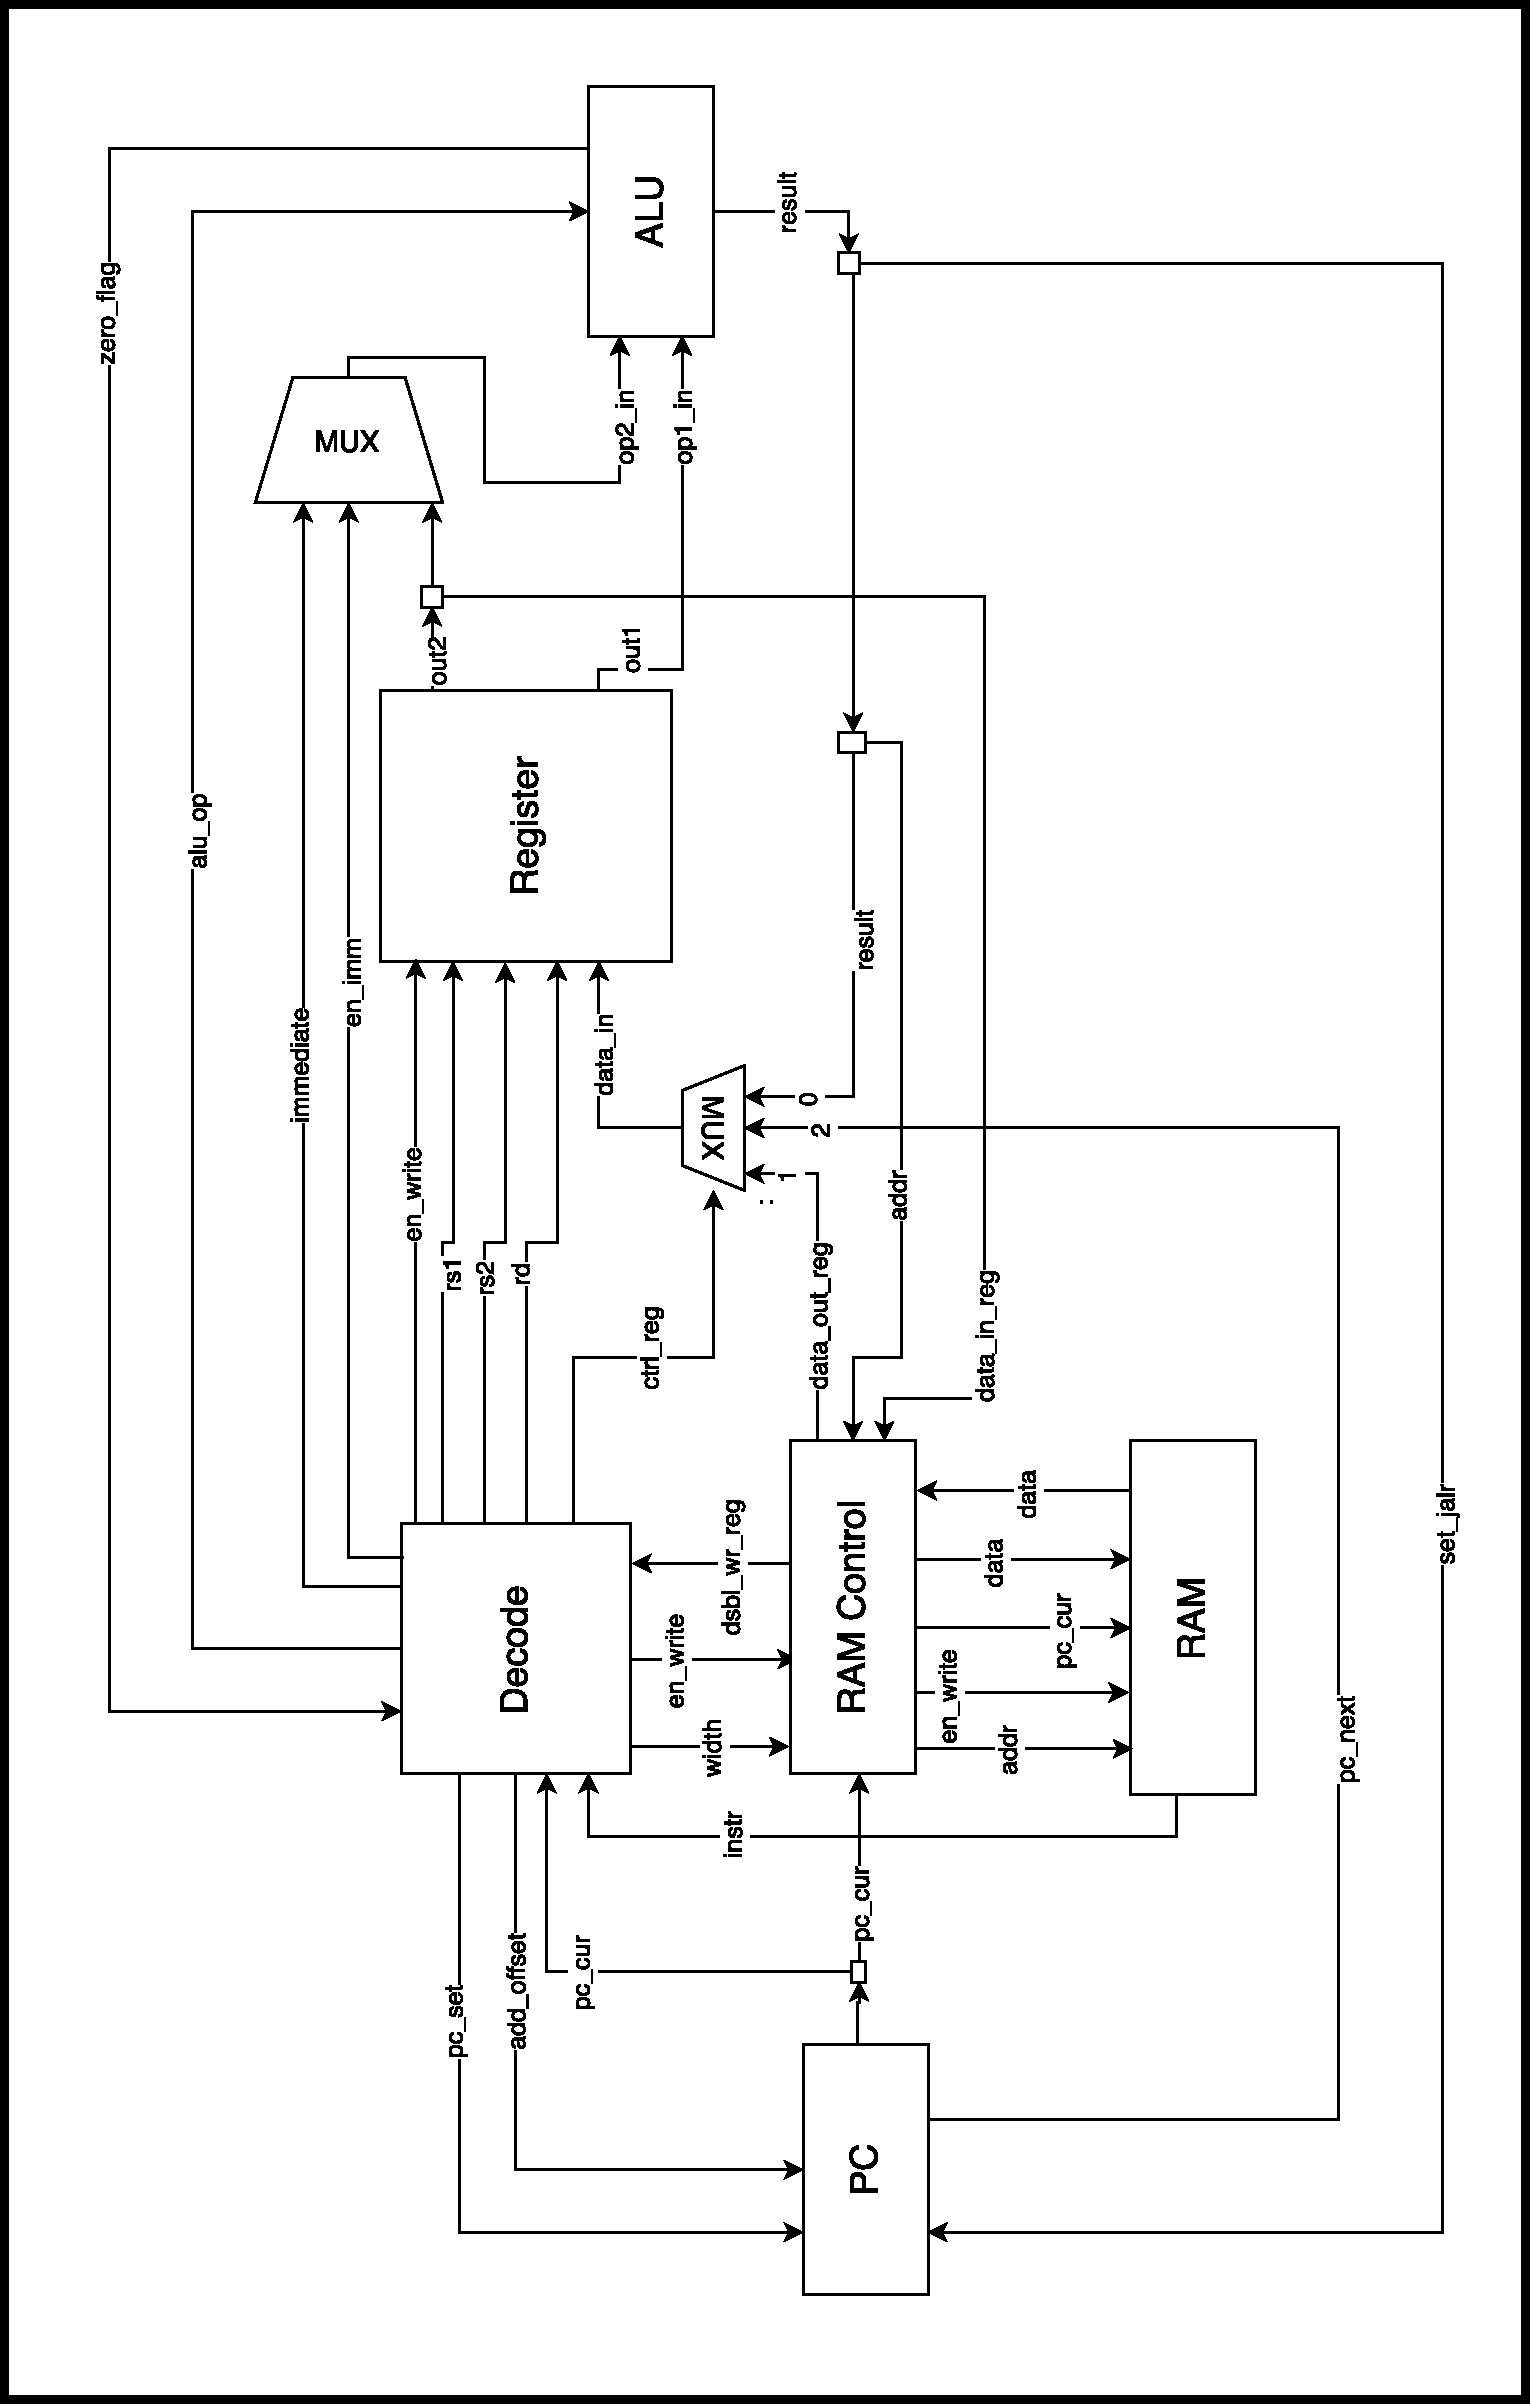
\includegraphics[width=\textwidth]{Figures/schaltplan.pdf}
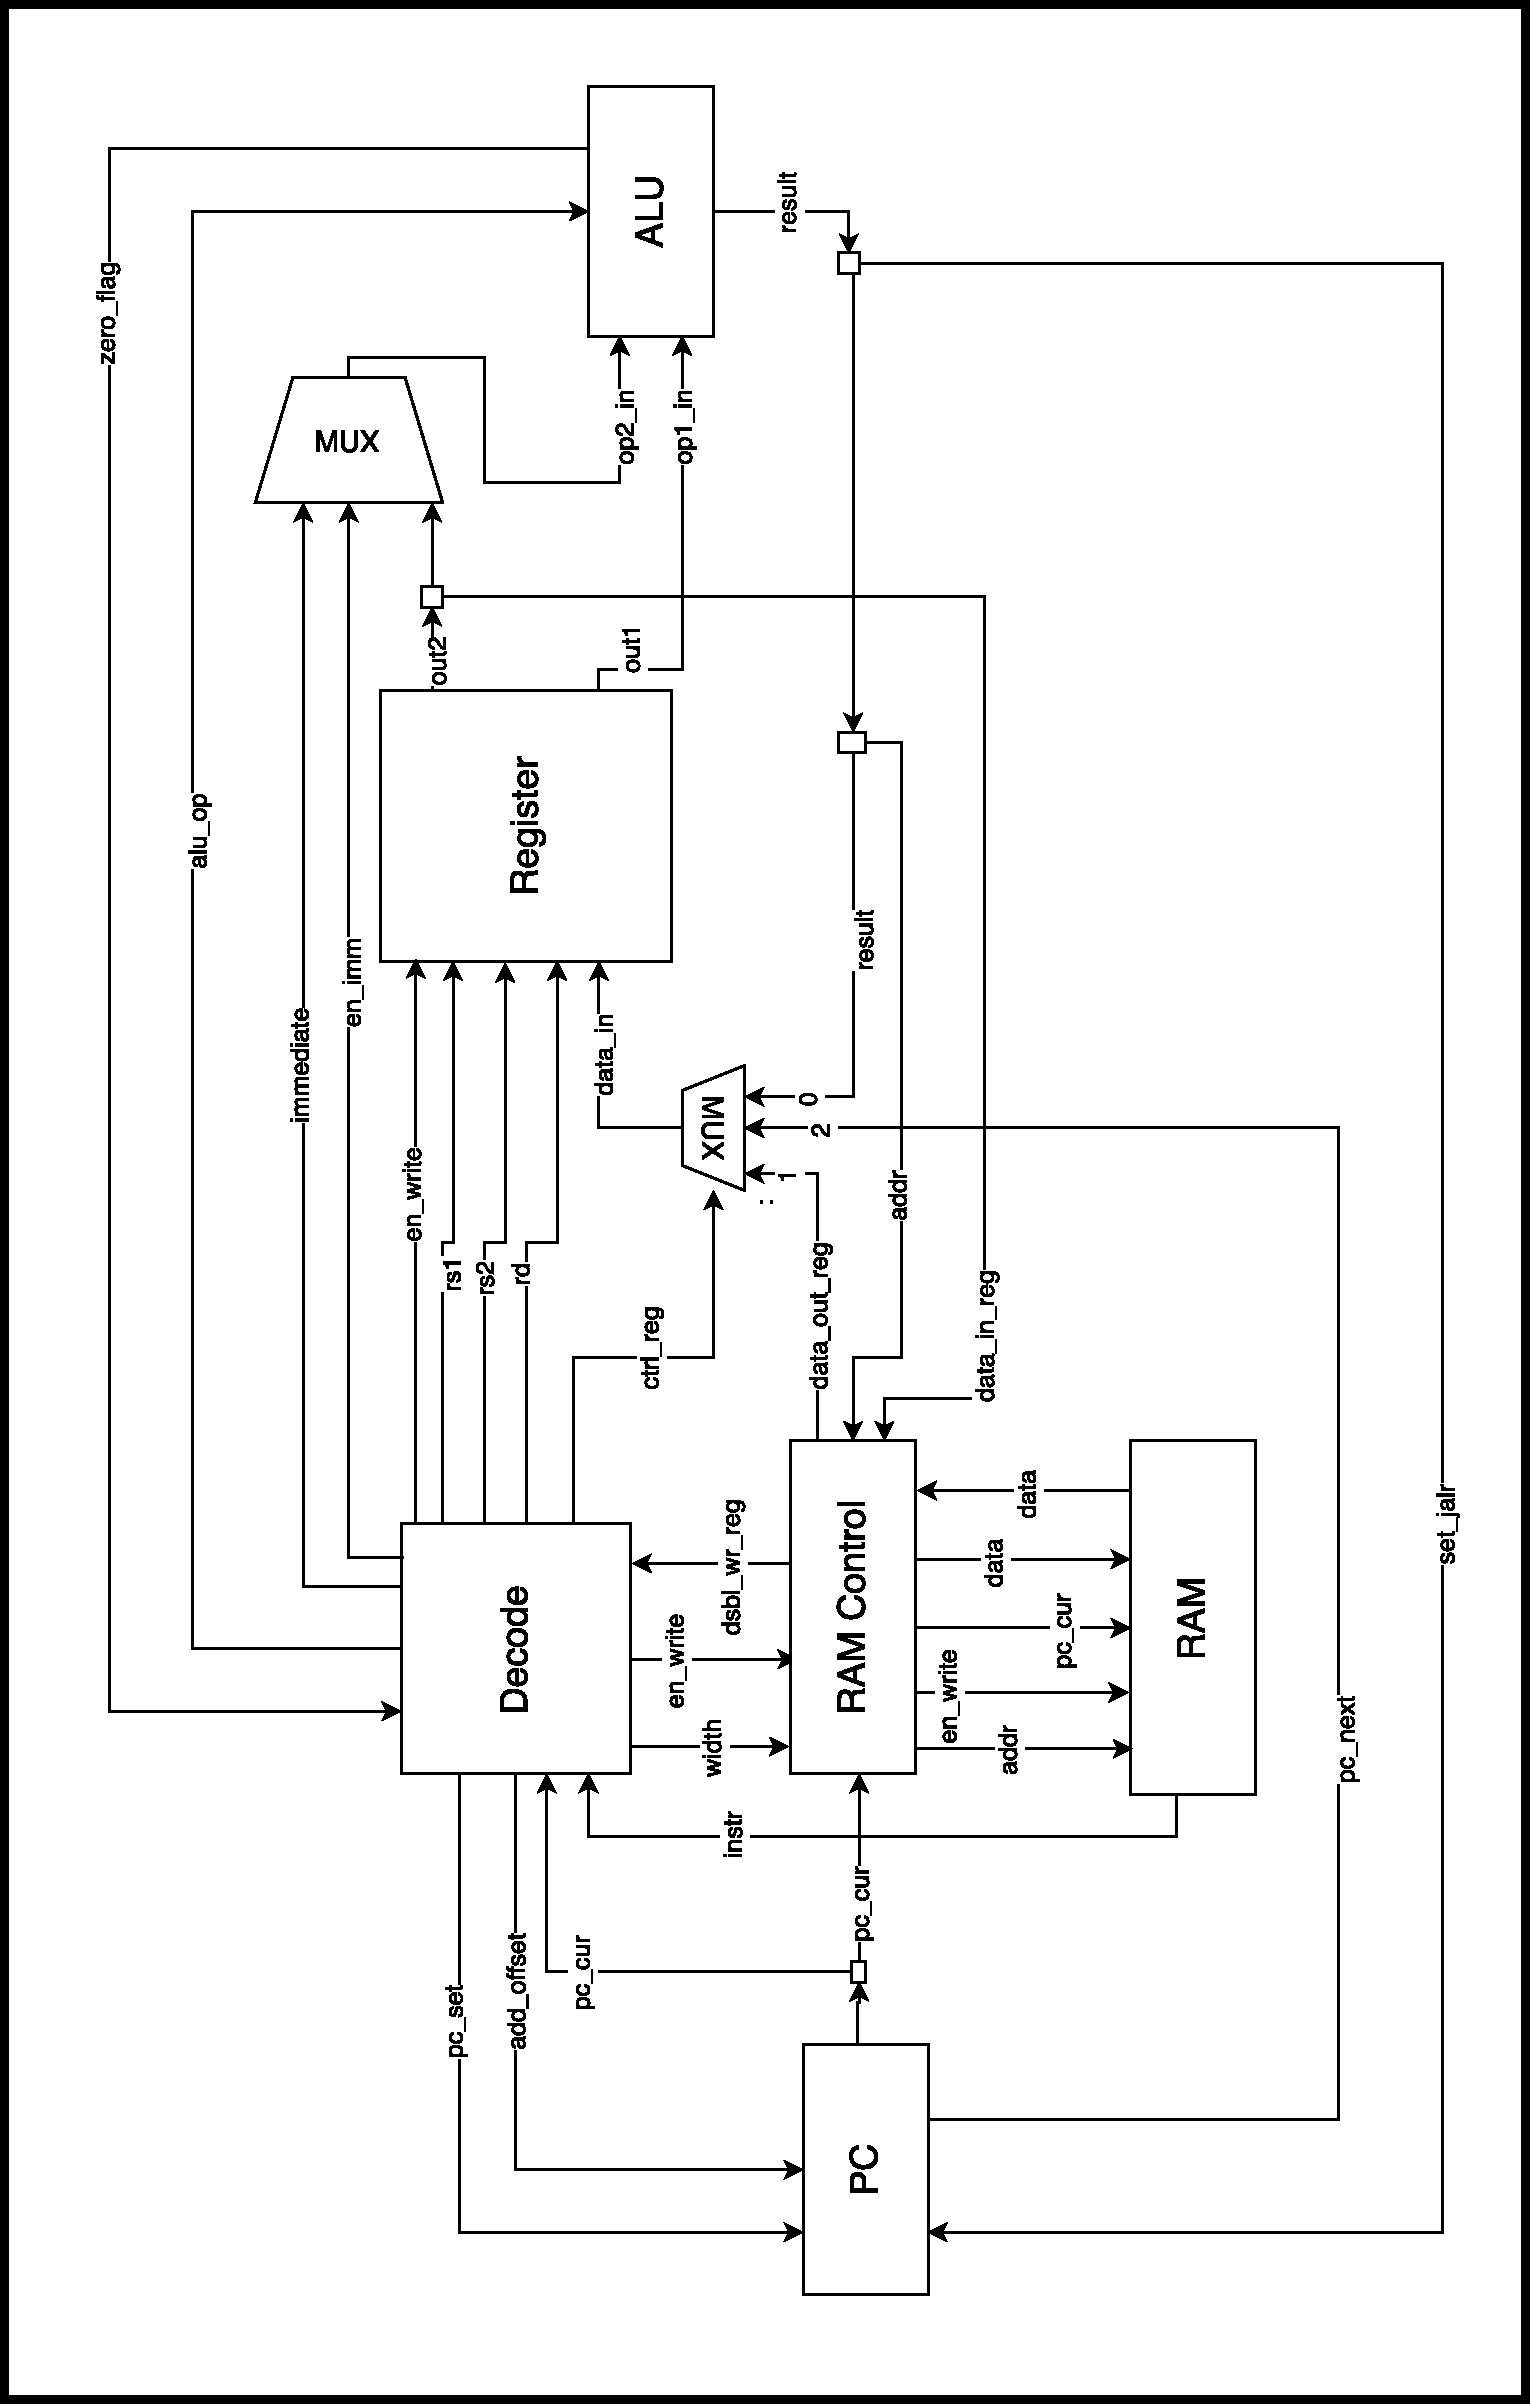
\includegraphics[height=0.8\textheight]{Figures/schaltplan.pdf}
%\end{figure}


\chapter{RISC-V Maschinenbefehle} % Main appendix title
\label{Maschinenbefehle} % For referencing this appendix elsewhere, use \ref{AppendixA}

\textbf{Liste der umgesetzten Maschinenbefehle aus der RV32I Instruktionsmenge}

\begin{center}
\includegraphics[width=1\textwidth]{RV32I_instr-1}
\end{center}
%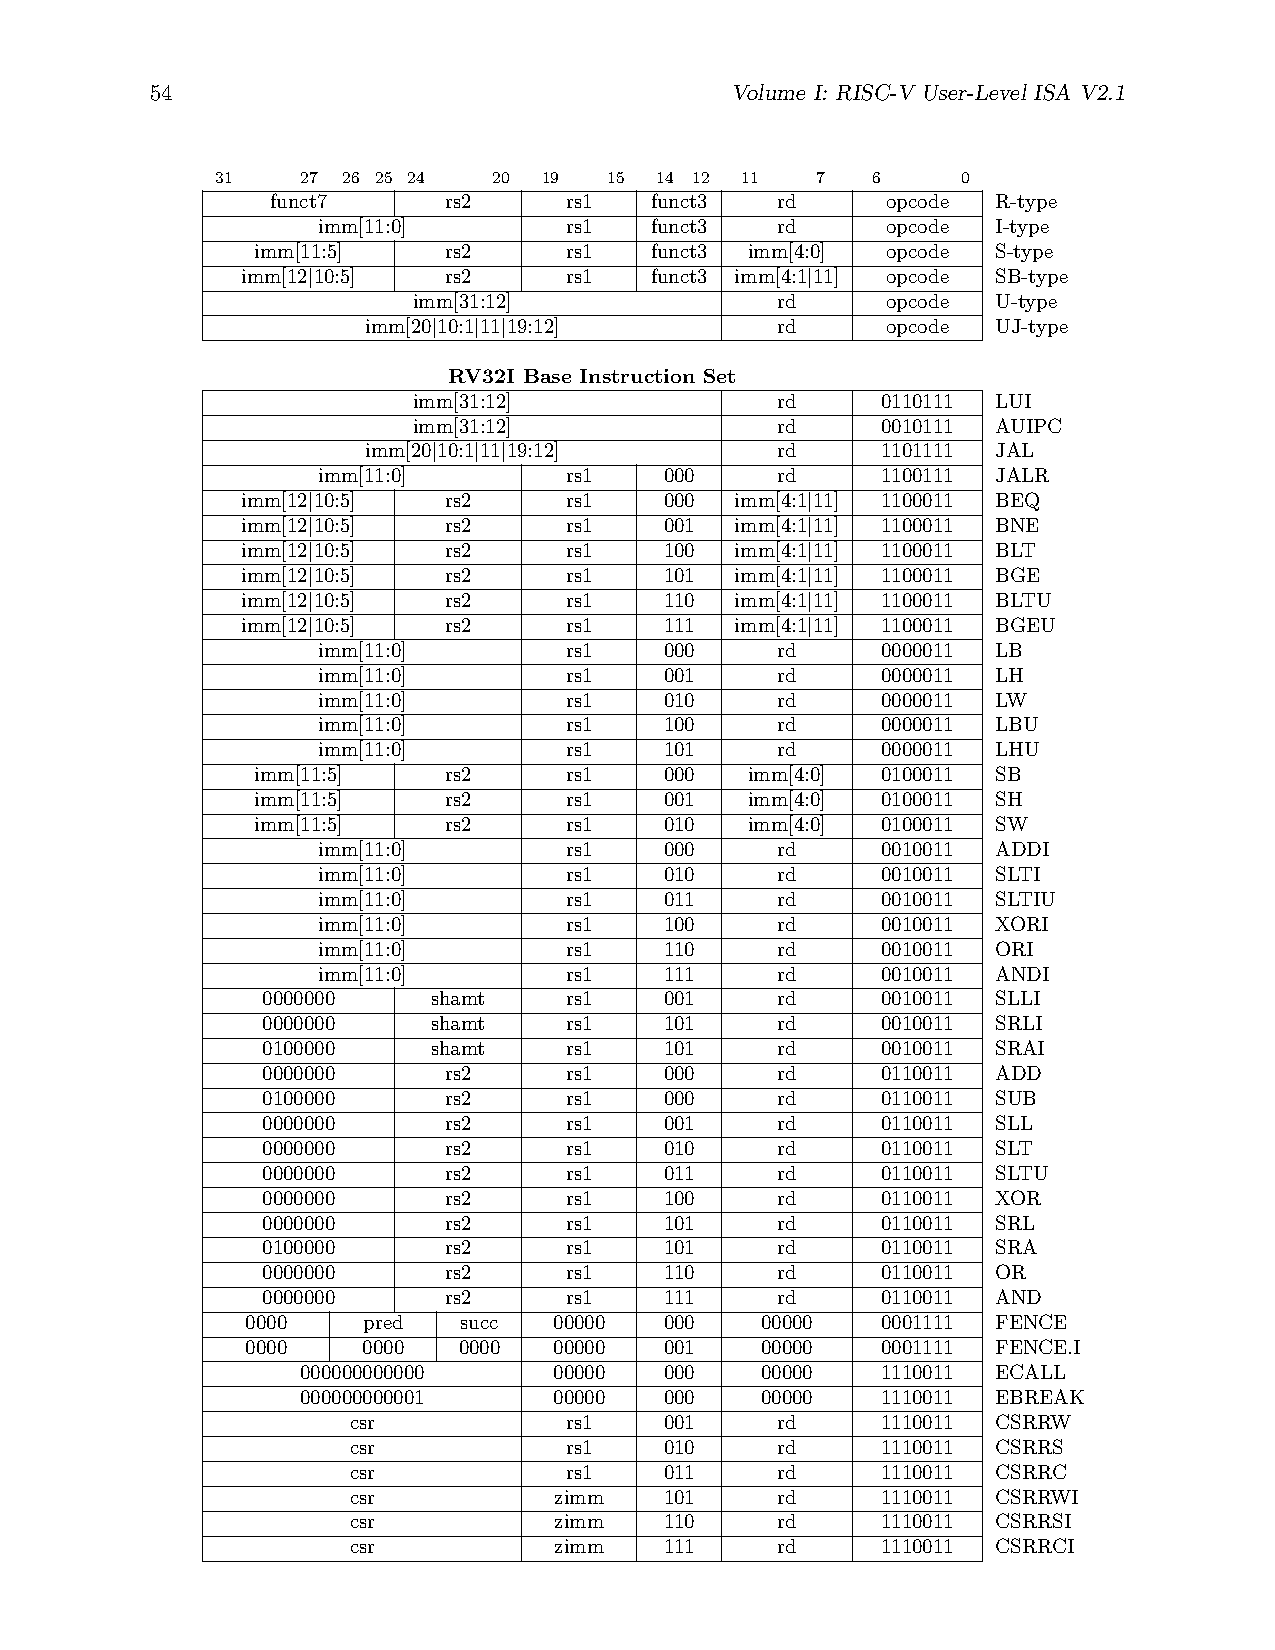
\includepdf[pages=-]{RV32I_instr}

Quelle: Auszug aus der RISC-V Spezifikation \cite[S. 54]{RISC}
%%% Appendix Template

\chapter{Quellcode} % Main appendix title

\label{quellcode} % Change X to a consecutive letter; for referencing this appendix elsewhere, use \ref{AppendixX}

\section{alu.vhd}
\label{src:alu.vhd}
\lstinputlisting[language=vhdl,tabsize=1, literate={\ \ }{{\ }}1]{../src/alu.vhd}


\section{block\_ram.vhd}
\label{src:block_ram.vhd}
\lstinputlisting[language=vhdl,breaklines,linerange={1-26,292-318}, tabsize=1, literate={\ \ }{{\ }}1]{\detokenize{../src/block_ram.vhd}}

\section{decode.vhd}
\label{src:decode.vhd}
\lstinputlisting[language=vhdl,tabsize=1, literate={\ \ }{{\ }}1]{../src/decode.vhd}

\section{main.vhd}
\label{src:main.vhd}
\lstinputlisting[language=vhdl,tabsize=1, literate={\ \ }{{\ }}1]{../src/main.vhd}

\section{mux.vhd}
\label{src:mux.vhd}
\lstinputlisting[language=vhdl,tabsize=1, literate={\ \ }{{\ }}1]{../src/mux.vhd}

\section{opcodes.vhd}
\label{src:opcodes.vhd}
\lstinputlisting[language=vhdl,tabsize=1, literate={\ \ }{{\ }}1]{../src/opcodes.vhd}

\section{pc.vhd}
\label{src:pc.vhd}
\lstinputlisting[language=vhdl,tabsize=1, literate={\ \ }{{\ }}1]{../src/pc.vhd}

\section{ram\_control.vhd}
\label{src:ram_control.vhd}
\lstinputlisting[language=vhdl,tabsize=1, breaklines,literate={\ \ }{{\ }}1]{\detokenize{../src/ram_control.vhd}}

\section{registerfile.vhd}
\label{src:registerfile.vhd}
\lstinputlisting[language=vhdl,tabsize=1, breaklines, literate={\ \ }{{\ }}1]{../src/registerfile.vhd}

\section{utils.vhd}
\label{src:utils.vhd}
\lstinputlisting[language=vhdl,tabsize=1, literate={\ \ }{{\ }}1]{../src/utils.vhd}

\section{main\_tb.vhd}
\label{src:main_tb.vhd}
\lstinputlisting[language=vhdl,tabsize=1, literate={\ \ }{{\ }}1]{\detokenize{../test/main_tb.vhd}}



%----------------------------------------------------------------------------------------
%	BIBLIOGRAPHY
%----------------------------------------------------------------------------------------

\printbibliography[heading=bibintoc]

%----------------------------------------------------------------------------------------

\end{document}  
